
\chapter{Aglomerado de Galáxias}
A origem do Universo, de acordo ao modelo cosmológico padrão, se deu há aproximadamente 14 milhões de anos. Desde então o seu processo de expansão ocorre de forma contínua e hierárquica, de modo que unidades menores se fundem formando outras maiores. Aglomerados de galáxias são as maiores estruturas do Universo observável e compõem os objetos de estudo desta dissertação.  

Aglomerados de galáxias são definidos basicamente por três componentes: galáxias, meio intra-aglomerado e matéria escura. A maior parte da massa do aglomerado, cerca de 80\% do total, é composta de matéria escura (não-bariônica). Do restante, na forma bariônica (feita de prótons e nêutrons), 15\% são compreendidos de gás intra-aglomerado (MIA) e apenas 5\% da massa de um aglomerado estão na forma de estrelas de galáxias.

A busca por compreender a formação e evolução dos aglomerados de galáxias é uma das questões mais importantes da Astrofísica. No paradigma atual de formação das estruturas, as galáxias e os aglomerados surgem a partir de halos escuros. O resfriamento desses halos ocasiona a formação de estruturas condensadas, onde depois colapsariam os bárions, formando  os sistemas astrofísicos conhecidos. Este cenário seria ainda hierárquico, com a formação dos aglomerados ocorrendo após a formação das galáxias, aproximadamente em um desvio para o vermelho $z \approx 2$ (Velásquez, 2007).
\begin{figure}[H]
	\centering
	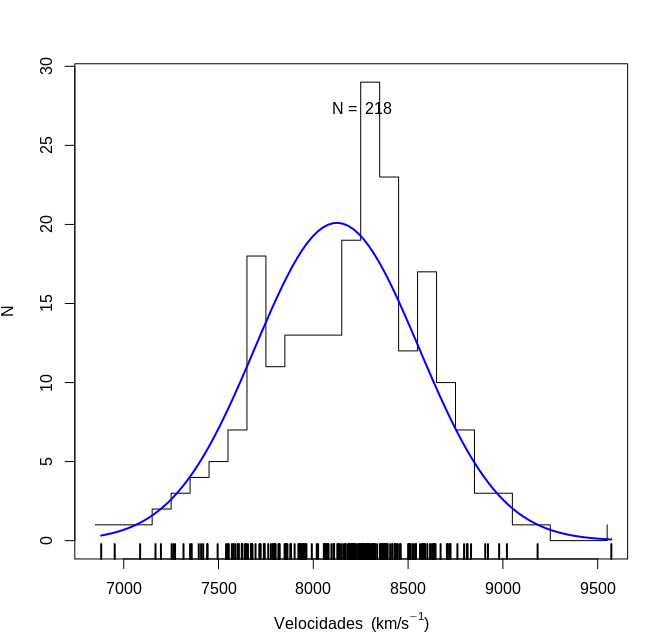
\includegraphics[width=0.5\textwidth]{04-figuras/10043dist}
	\caption{Histograma de velocidades no Aglomerado.}
	\textbf{Fonte: Autor.}
	\label{fig1}
\end{figure}

O processo de formação de aglomerados de galáxias ainda não atingiu o seu fim. Enquanto regiões centrais estão em equilíbrio dinâmico, as regiões periféricas (externas) acumulam matéria na forma de galáxias ou grupos de galáxias de modo contínuo. Comumente o entorno dos aglomerados de galáxias é constituído de grupos de galáxias que podem ser absorvidos pelo aglomerado principal ao longo do tempo, ocasionando o aumento de sua massa \cite{rembold2011}. Estudos sobre a distribuição de velocidades de galáxias em aglomerados indicam que a mesma possui distribuição Não Rejeita, vide Figura \ref{fig1}, ou muito bem ajustada por uma gaussiana somente na região virializada do sistema (região mais interna do sistema) \cite{yahil1977velocity}, podendo existir sinais de múltiplos modos normais na região mais externa \cite{ribeiro2011non}, comprovando a presença de componentes de um sistema em processo de evolução pelo acréscimo de matéria ao seu entorno. Esse acréscimo de matéria, na forma de galáxias ou grupo de galáxias.  Isto sugere que a formação de aglomerados de galáxias é um processo contínuo que decorre de fusões sucessivas e encontros gravitacionais de maiores e menores proporções \cite{nascimento2016dynamical}.


\section{Distribuição de Velocidades ao longo do Aglomerado}
A velocidade de uma galáxia contida em um aglomerado, em uma dada posição, não pode ser maior que a velocidade de escape do sistema, caso isto aconteça a galáxia não pertenceria mais ao aglomerado. A velocidade de escape e a distância ao centro do aglomerado são grandezas inversamente proporcionais, ou seja, a velocidade de escape decresce com o aumento da distância ao centro do aglomerado, portanto é mais fácil o escape de uma galáxia que está na região periférica (de Oliveira e Viegas, 2004).

Para que o aglomerado exista como unidade dinâmica é preciso uma redução na amplitude da distribuição de velocidades das galáxias à medida que haja um afastamento da região central. O grande problema dessa propriedade é o efeito de projeção. As galáxias que estão com distâncias distintas do centro do aglomerado podem parecer ao observador com mesma distância em consequência da observação apenas das posições projetadas no plano do céu (de Oliveira e Viegas, 2004).

Na Figura \ref{fig2} vemos a distribuição de velocidades do aglomerado em função da distância da galáxia ao centro do aglomerado, onde o estreitamento da distribuição de velocidades define uma espécie de "corneta" que pode ser utilizada para definir os membros de um aglomerado, sendo removidas as galáxias que estejam significativamente acima ou abaixo da "corneta".

\begin{figure}[H]
	\centering
	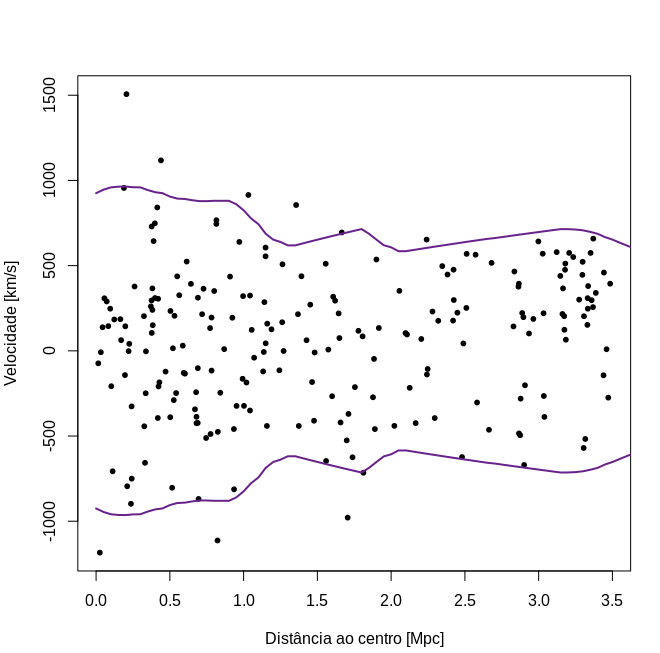
\includegraphics[width=0.5\textwidth]{04-figuras/10043}
	\caption{Distribuição de velocidades em função da distância ao centro do Aglomerado.}
	\textbf{Fonte: Autor.}
	\label{fig2}
\end{figure}

\chapter{Rotação de Aglomerados}

O conhecimento do estado dinâmico de aglomerados de galáxias pode propiciar restrições importantes em cenários cosmológicos, como a determinação da massa total do aglomerado e uma estimativa da quantidade de matéria escura no Universo. A possibilidade da existência de aglomerados em rotação tem sido discutida por muitos autores (por exemplo, veja os estudos de \cite{hwang2007searching, manolopoulou2016galaxy}). 

Para detecção de indícios de rotação, \citeonline{hwang2007searching} utilizaram dados espectroscópicos do \textit{Sloan Digital Sky Survey} \footnote{Considerado o mais ambicioso mapeamento astronômico que já foi feito. Com este mapeamento, os astrônomos podem observar os padrões de grande escala das galáxias: filamentos e vazios em grandes regiões angulares do Universo.}(SDSS) e \textit{Two-Degree-Field Galaxy Redshift Survey} (2dF-GRS). A rotação de aglomerados foi modelada como a rotação de galáxias membro e a rotação do gás intra-aglomerado. Eles levantaram inicialmente a hipótese de que a rotação se origina através de fusões de aglomerados. Um aspecto importante do método empregado por \citeonline{hwang2007searching} é que os aglomerados com rotação devem exibir divisão espacial entre galáxias com velocidades maiores e menores que a velocidade média do aglomerado além de apresentar um pico no mapa de densidade. Nesta pesquisa de \citeonline{hwang2007searching} foram detectados seis sistemas com rotação, em um total de dozes aglomerados (Abell 0954, Abell 1139, Abell 1399, Abell 2162, Abell 2169, and Abell 2366). Constatou-se ainda que estes aglomerados estão em equilíbrio dinâmico e não sofreram fusão recente, não dando suporte, portanto, à hipótese de interações como causadoras da rotação. 

\citeonline{kalinkov2005rotation} tentaram obter o gradiente máximo no campo de velocidades de Abell 2107 e determinaram que a direção do coeficiente de correlação linear máximo definiria o eixo maior do aglomerado e o eixo menor seria o de rotação. Foram utilizadas subamostras de galáxias membro, ordenadas de acordo a distância ao centro do aglomerado para definir o grau de rotação do sistema. Esse mesmo aglomerado foi estudado por \citeonline{oegerle1992structure} e foram encontrados indícios de rotação. \citeonline{materne1983cluster} apontaram a dificuldade em diferenciar um aglomerado rotativo de dois que se sobrepõem, pelo motivo de estar se fundindo ou se afastando. Porém, o aglomerado  Abell 2107 não consiste de dois aglomerados sobrepostos, em consequência do pico estreito representado em seu histograma de velocidades. O indicador mais forte que definiu a rotação foi o ângulo de posição do eixo com o gradiente máximo no campo de velocidades quase coincidindo com o ângulo de posição do eixo com o maior alongamento.  Nesse estudo o período de rotação foi calculado em uma volta a cada $2.4\times10^9$ anos e houve uma correção no valor da massa para $2.8\times10^{14}~{M_\odot}$  (a massa inicial era de $3.2\times10^{14}~{M_\odot}$, sem levar em conta a rotação). 

Baseado no estudo da distribuição de velocidades das galáxias membro, \citeonline{tovmassian2015rotation} detectou
sinais de rotação em 17 de uma amostra de 65 aglomerados (26\%).
O método analisa o número de galáxias com velocidades mais baixas e mais altas que a velocidade média do aglomerado em diferentes partes do aglomerado. O método teve mais êxito em aglomerados planos, com $f=a/b > 1.8$ (a e b semieixos - maior e menor – da distribuição de galáxias do aglomerado). 
Para estes, a taxa de detecção de rotação foi mais alta (7 dos 18 aglomerados planos, 39\%).  Esse resultado suporta a opinião de que os aglomerados foram originalmente formados a partir das enormes nuvens de gás primordiais e preservaram a rotação das nuvens primordiais, a menos que sofram fusões com outros aglomerados e grupos de galáxias. 

Já na tese de \citeonline{manolopoulou2016galaxy} é realizado um estudo de um novo algoritmo para dedução de rotação usando a velocidade radial projetada\footnote{É a velocidade de um objeto na direção da linha de visada, isto é, a velocidade com que o objeto se aproxima ou se afasta do observador.}. Inicialmente os testes foram realizados em aglomerados gerados em simulações de Monte Carlo para confirmar se o método fornecia indicações robustas de rotação. Em seguida, aplicado em amostras de aglomerados de Abell. Através do teste de Kolmogorov-Smirnov, decidiu-se quanto a sua rotação significativa ou não, seu centro rotacional, orientação do eixo de rotação, amplitude de velocidade rotacional e, finalmente, o sentido de rotação no sentido horário ou anti-horário no plano do céu. Foram encontrados 23 aglomerados possivelmente rotativos dentro de 1.5 Mpc ou a uma distância de 2.5 Mpc do centro do aglomerado, do total de 45 da amostra.

\citeonline{nascimento2016dynamical}, a partir de uma amostra de galáxias observadas no Cerro Tololo Interamerican Observatory (CTIO), realizaram um estudo dinâmico em torno do par de aglomerados de Abell (A3407 e A3408). O objetivo era verificar se a amostra correspondia a um simples sistema de galáxias ou a um processo de fusão, melhorando o entendimento desse sistema. Testes estatísticos foram aplicados aos membros mostrando que ambos os sistemas bem como cada aglomerado individual tem uma distribuição de velocidade Gaussiana. Um gradiente de velocidade de $\approx 847 \pm 114\; {km~s^{-1}}$ foi identificada ao redor do eixo principal da distribuição de galáxias projetada indicando uma possível rotação. 
O estudo definiu um "gap" na distribuição de velocidades e realizou testes sobre a distribuição espacial de galáxias (em torno do eixo principal do aglomerado) visando identificar diferenças entre objetos com velocidades maiores e menores que a posição do "gap". Esta comparação indicou que havia diferença significativa entre estas subamostras, sugerindo um grau de rotação no sistema A3407+A3408 (vide Figura \ref{fig3}).

\begin{figure}[H] %h or !htbp
\vspace{-2pt}
\begin{center}
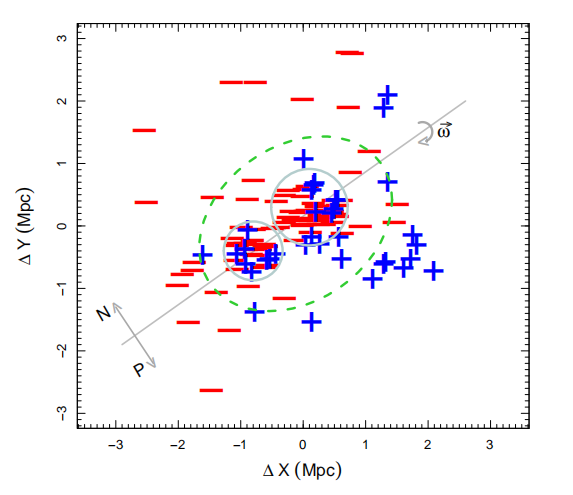
\includegraphics[height=9cm,width=9cm]{04-figuras/nascimento.png}%
\caption{Distribuição de galáxias no plano do céu do par de aglomerados A3407 e A3408.}
 \textbf{Fonte: Nascimento et al. 2016.}
\label{fig3}%
\end{center}
\end{figure}

\chapter{Ferramentas Estatísticas Utilizadas}
\section{Teste de Hipótese}
A análise estatística objetiva, especialmente, fazer inferência sobre uma população a partir da observação de uma amostra. Os testes de hipótese representam uma forma de inferência estatística. A hipótese é uma afirmação sobre parâmetros populacionais que devem ser analisadas para verificar sua veracidade. É importante ressaltar que a verdade ou não nunca pode ser determinada, a menos que toda a população seja observada, situação impraticável na maioria das vezes, justificado pelo uso do teste estatístico.  

A princípio é necessário estabelecer como verdadeira a \textbf{hipótese nula}, denotada por \textbf{$H_0$}. Já a \textbf{hipótese alternativa ($H_1$)}, contrapõe a hipótese nula, ou seja, $H_0$ deverá ser rejeitada. É necessário estabelecer um critério auxiliar para decidir a rejeição ou não de $H_0$ para um teste estatístico. Esse valor, determinado pelo pesquisador antes da análise de dados ou até mesmo na coleta de dados, cenário ideal, é denominado \textbf{nível alfa ($\alpha$) ou nível de significância}. Comumente é utilizado como critério de rejeição uma probabilidade de 5\%. De acordo com \citeonline{cramer2004sage}, 

\begin{citacao}
O nível em que a hipótese nula é rejeitada é geralmente definido como 5 ou menos vezes fora de 100. Isso significa que tal diferença ou relacionamento é provável que ocorra por acaso 5 ou menos vezes de 100. Este nível é geralmente descrito como proporção 0.05 e às vezes como a porcentagem 5\%. O nível de probabilidade de 0.05 foi historicamente uma escolha arbitrária, mas tem sido aceitável como uma escolha razoável na maioria das circunstâncias. Se houver um motivo para variar este nível, é aceitável fazer então. Então, em circunstâncias em que pode haver consequências adversas muito graves se a decisão errada foi feita sobre a hipótese, então o nível de significância poderia ser mais rigoroso em, digamos, 1\% \cite[p.~151]{cramer2004sage}. 
\end{citacao}

Na realização de testes de hipóteses é possível que erros sejam cometidos, como mostrado no quadro \ref{qua:hipotese}. \textbf{Erro do tipo I}, denotado por \textbf{erro $\alpha$}, a rejeição de $H_0$ quando ela é verdadeira. Contrapondo, a não-rejeição de $H_0$ quando esta é falsa é denominada \textbf{erro do tipo II} e representado por \textbf{$\beta$}.  Esse tipo de teste permite concluir se deve aceitar ou rejeitar a hipótese nula, porém não é possível quantificar o quão provável é o resultado de ocorrer ao acaso. Apoiado por isto, é definido a potência de um teste estatístico $1-\beta$ como a probabilidade de rejeitar $H_0$ quando de fato é falsa. Claramente, o teste ideal é aquele em que os valores de $\alpha$ e $\beta$ são mínimos. Porém, o valor de $\alpha$ é inversamente relacionado com o valor de $\beta$, sendo impossível minimizá-los simultaneamente. Geralmente, é fixado o nível de significância $\alpha$ e escolhido a região de rejeição que minimiza $\beta$, ou seja, que maximize a potência do teste. 


\begin{quadro}[!htb]
	\centering
	\caption{Tipos de erros em testes de hipótese.\label{qua:hipotese}}
	\begin{tabular}{|l|l|l|ll}
		\cline{1-3}
\multicolumn{1}{|c|}{\multirow{2}{*}{\textbf{Decisão Estatística}}} & \multicolumn{2}{l|}{\textbf{Natureza (estado verdadeiro ou desconhecido)}} &  &  \\ \cline{2-3}
\multicolumn{1}{|c|}{} & \multicolumn{1}{c|}{\textbf{$H_0$ verdadeira}} & \multicolumn{1}{c|}{\textbf{$H_1$ falsa}} &  &  \\ \cline{1-3}
\textbf{Aceitar $H_0$} & acerto & Erro tipo II ( \ensuremath{\beta}) &  &  \\ \cline{1-3}
\textbf{Rejeitar $H_0$} & Erro tipo I ( \ensuremath{alpha}) & acerto &  &  \\ \cline{1-3}
	\end{tabular}
	\fonte{\citeonline{}}
\end{quadro}

O menor nível de significância pode ser definido utilizando o \textbf{valor-p} ou \textbf{\textit{“p-value”}}. No teste de hipótese esse valor é comparado ao nível de significância \ensuremath{alpha} determinado no início objetivando a tomada de decisão de aceitar ou rejeitar $H_0$. Se o valor-p calculado do teste for igual ou maior que \ensuremath{alpha}, a $H_0$ é aceita. Ou seja, a hipótese nula é consistente com os resultados da amostra. Porém, se o valor-p for menor que \ensuremath{alpha}, a hipótese nula é rejeitada, a hipótese alternativa, nesse caso, é então aceita como verdadeira.

\section{Teste de Normalidade}
Uma variável aleatória, seja idade de um grupo de pessoas ou ocorrência de um determinado desfecho, pode admitir uma distribuição de frequências da população, contendo diversas formas encontradas na literatura estatística. O intuito desses modelos é caracterizar o comportamento de um determinado evento em função da frequência de sua ocorrência. Se as variáveis forem contínuas, o evento será um intervalo de valores. Portanto, as distribuições de frequências são efetivamente distribuições de probabilidade, em que para um evento teremos associado uma probabilidade de ocorrência (T2). 

A inspeção visual pode ser utilizada para avaliação da normalidade. A distribuição de frequência, como exemplo um histograma, relaciona valores observados à sua frequência e pode além de pressupor uma distribuição normal, identifica \textit{insights} sobre lacunas nos dados e outliers. O histograma é composto por barras justapostas em que no eixo horizontal contém a variável de interesse dividida em classes e no eixo vertical a sua correspondente frequência (T2). Para distribuições do tipo normal ou Gaussiana, o histograma constitui formato de sino (Figura 3b).

Entretanto, a simples constatação por meio de gráficos é subjetiva e não satisfatória, pois depende de uma interpretação visual além de não ser confiável no caso multivariado e especificamente nas situações de muitas variáveis. Desta forma, para inferir sobre a normalidade é necessário utilizar como complemento testes estatísticos (T1).  Como exemplo, podemos citar: o teste de aderência qui-quadrado; Kolmogorov-Smirnov; Lilliefors e Shapiro-Wilk. 

Estes testes possuem estatísticas de teste e critérios de decisão diferentes, porém compartilham da hipótese avaliada: a hipótese de nulidade ($H_0$) especifica que a variável aleatória adere à distribuição normal, sem a necessidade de definir a média ou variância da distribuição. Já a hipótese alternativa ($H_1$), opõe a hipótese nula (T2). 

O resultado que interessa após executar um determinado teste é o seu valor-p ou nível descritivo do teste, referente à probabilidade de que a estatística do teste (como variável aleatória) tenha valor extremo em comparação ao valor observado (estatística) quando a hipótese nula é verdadeira. Sendo o valor-p menor que o nível de significância, logo a hipótese nula é rejeitada. Ou seja, o valor-p representa o menor nível de significância que pode assumir para então rejeitar a hipótese nula. Logo, há significância estatística quando o valor-p é menor que o nível de significância estabelecido \cite{FLAVIO2012}.  

\section{Testes de duas amostras}
O teste de duas amostras é uma análise estatística projetada para utilizar dados de duas amostras aleatórias. O intuito do teste é determinar se a diferença entre as duas populações é estatisticamente significativa. 

Seja $X_1, X_2, ..., X_m$ e $Y_1, Y_2, ..., Y_N$ duas amostras aleatórias independentes com funções de distribuição contínua F e G, respectivamente, o teste de duas amostras verifica se

\begin{equation}
 H_0 : F = G  \hspace{2cm} H_1 : F \neq G
\label{eq:twoSample}
\end{equation}

Isto é, assume como hipótese nula que as médias populacionais das amostras não são significativamente diferentes.

\section{Testes utilizados}
\subsection{Teste de Cramer-von Mises}
Em estatística, o teste de Cramér (conhecido também como phi de Cramer - $\varphi$c) é uma medida de associação entre duas variáveis nominais dado o intervalo de 0 a 1, indicando que um valor mais alto possui forte associação. Fundamentado no teste estatístico do qui-quadrado de Pearson, foi publicado em 1946 por Harald Cramér. A medida é definida como

\begin{equation}
\ V = \sqrt{\frac{{\chi_{obt}}^2}{N.m}}
\label{eq:eq1}
\end{equation}
	
	onde $\chi^2$ é o valor obtido do teste estatístico
	
	N é o tamanho da amostra e 
    
    m = o menor de (r - 1) ou (c – 1), sendo r o número de linhas e c o número de colunas.

Para entender melhor a utilidade do teste de Cramer é fundamental compreender as formas como os testes estatísticos divergem das medidas de associação para variáveis categóricas. O teste qui-quadrado ($\chi^2$) fornece um teste estatístico de associação entre duas variáveis categóricas (nominais) de uma população única. Ele determina se a associação entre as variáveis é significativa, utilizando como hipótese nula ($H_0$) que as duas variáveis não são dependentes uma da outra e como hipótese alternativa ($H_1$) é que existe alguma associação entre duas variáveis.

O teste de Cramer é considerado um dos favoritos entre as medidas baseadas no qui-quadrado. Geralmente, quando o seu cálculo resulta no valor máximo 1 é que exista um forte relacionamento entre duas variáveis. No cálculo de Cramer é levado em consideração as dimensões da tabela, ou seja, diferentes dimensões podem ser comparadas significativamente.

\subsection{Teste de Hotelling}

Um dos mais conhecidos testes de hipóteses multivariados foi proposto por Harold Hotelling em 1947, o teste de $T^2$, compara vetores de médias populacionais. Baseado na generalização da estatística \textit{t de Student}, foi o primeiro a levar em consideração a correlação das variáveis na formulação da estatística do teste.

Sendo \textbf{\textit{X}} um vetor aleatório com uma dada dimensão, \textbf{\textit{$\mu$}} o vetor de médias e \textbf{\textit{$\sigma$}} a matriz de covariância. Para \textbf{\textit{X}}, sendo uma distribuição Não Rejeita multivariada e com tamanho de amostra aleatória \textbf{\textit{n}}, a estatística de $T^2$ é dada por
\begin{equation}
\ T^2 = n(\overline{X} - \mu_0) \sum_{pxp}^{-1} {(\overline{X} - \mu_0)}
\label{eq:eq2}
\end{equation}

com

\begin{equation}
 H_0 : \mu = \mu_0 \hspace{2cm} H_1 : \mu \neq \mu_0
\label{eq:eq3}
\end{equation}

A equação \ref{eq:eq2} tem distribuição qui-quadrado com \textit{p} graus de liberdade. Definindo um nível de significância $\alpha$, com $0 < \alpha < 1$, para valores de $T^2$  maiores ou iguais ao valor crítico ${\chi^2_{a,p,c}}$ dado por $P[{\chi_p}^2 \geq {\chi^2_{a,p,c}}]$,  a hipótese nula será rejeitada.   

Sendo a matriz desconhecida, a estatística de $T^2$ é dada por

\begin{equation}
T^2 = n(\overline{X} -\mu_0) S^{-1}(\overline{X} - \mu_0)
\label{eq:eq4}
\end{equation}

que sob a hipótese nula, tem uma distribuição proporcional a uma distribuição F, ou seja, o valor crítico do teste a um nível de significância $\alpha$, com $0 < \alpha < 1$, é

\begin{equation}
F_c = \frac{p(n-1)}{n-p} F_{1-\alpha, p, n - p}
\label{eq:eq5}
\end{equation}

onde $F_{1-\alpha, p, n - p}$ é a probabilidade acumulada igual a (1 - $\alpha$) da distribuição de F com p
n-p é igual a graus de liberdade.

Sendo S a matriz de covariâncias amostrais (\textit{pxp}), um estimado não viciado de $\sum_{pxp}$, dado por
\begin{equation}
\begin{bmatrix}
S^{2}_{1} & S_{12} & ... & S_{1p} \\ 
 & S^{2}_{2} & ... & S_{2p} \\ 
 &  & \ddots  & \vdots  \\ 
 &  &  & S^{2}_{p}
\end{bmatrix}
 \label{eq:eq6}
\end{equation}

em que os elementos da diagonal principal de S são as variâncias definidos por
\begin{equation}
S^2_j = \frac{1}{m-1} \sum_{k=1}^m (x_{jk} - \overline{X}_j),    j = 1, 2, ..., 3 
\label{eq:eq7}
\end{equation}

e os elementos fora da diagonal principal são as covariâncias conforme

\begin{equation}
S_{jh} = \frac{1}{m-1} \sum_{k=1}^m (x_{jk} - \overline{X}_j)(x_{hk} - \overline{X}_h) 
\label{eq:eq8}
\end{equation}

onde $x_{jk}$ e $x_{hk}$ representam os valores amostrais das variáveis $X_j$ e $X_h$.

\chapter{Linguagem R}

R é uma linguagem e ambiente para análise estatística e produção de gráficos, desenvolvida na década de 90 pelos estatísticos Ross Ihaka e Robert Gentleman que utilizavam sistemas pagos em seus projetos. Contém diversos pacotes integrados permitindo que sejam realizadas uma grande variedade de estatísticas (natureza linear, não-linear, séries temporais) e o uso de recursos gráficos avançados, o que a distingue das demais linguagens. 

O R é um conjunto integrado de instalações de software para manipulação de dados, cálculos e exibição gráfica. Isto abrange uma instalação eficaz de manipulação e armazenamento de dados, um conjunto de operadores para cálculos em matrizes, uma grande coleção coerente de ferramentas intermediárias para análise de dados e representações gráficas, a inclusão de condicionais (\textit{loops} e funções recursivas) definidas pelo usuário e recursos de entrada e saída.  

\section{Pacotes}

\subsection{Pacote Cramer}
Uma rotina em R aplicada para o teste de Cramer de duas amostras. O valor de retorno é um objeto da classe \textit{"cramertest"}, contendo, dentre outros, os seguintes componentes:

\begin{itemize}
   \item \textit{\textbf{statistic}}: valor estatístico do teste de Cramer para observações.
   \item \textit{\textbf{conf.level}}: nível de significância do teste.
   \item \textit{\textbf{p.value}}: estimativa do valor-p.
 \end{itemize}  

\subsection{Pacote Hotelling}
Uma rotina em R aplicada para o teste de Hotelling de duas amostras. O valor de retorno é uma lista da classe \textit{"’hotelling.test"}, contendo, dentre outros, o seguinte componente:

\begin{itemize}
   \item \textit{\textbf{pval}}: estimativa do valor-p.
 \end{itemize} 


\subsection{Pacote Ellipse}

Este pacote contém diversas rotinas para desenhar elipses e regiões de confiança do tipo elipse, implementando os gráficos descritos por Murdoch e Chow (1996) e Bates e Watts (1988).


\subsection{Pacote Astro}

O pacote \textbf{astro} fornece uma série de funções, ferramentas e rotinas no uso diário da astronomia. Pode-se agrupar essas funções em áreas como a cosmologia \footnote{Funções que calculam distâncias, movimentação de volumes, \textit{lookback time} e luminosidade em uma cosmologia plana}, manipulação de arquivos FITS \footnote{Sistema flexível de transporte de imagens (\textit{Flexible Image Transport System}), um formato de arquivo comum em astronomia}, funções de tempo e posição.

\subsection{Pacote cosmoFns}
 O pacote contém expressões de distância, tempo, luminosidade e outras úteis na cosmologia observacional, compreendendo observações em linhas moleculares. Atualmente codificado apenas para o universo plano.

\chapter{Dados e Metodologia}

O método proposto por Nascimento et al. (2016) para estudar um par de aglomerados pode ser adaptado para o estudo da rotação de aglomerados individuais. Neste trabalho fazemos esta adaptação e a implementamos em linguagem R. O código resultante é aplicado a um conjunto de três catálogos: 

\begin{itemize}
   \item \textit{\textbf{Catálogo I: }} composto por 20 aglomerados ricos do SDSS, localizados em baixos $redshifts$, com espectroscopia disponível para objetos com $m_r \leq 17.77$.
   \item \textit{\textbf{Catálogo II: }} NoSOCS (\textit{\textbf{Northern Sky Optical Cluster Survey}}) com baixo redshift ($z \leq 0.10$), compreendendo 183 objetos.	
   \item \textit{\textbf{Catálogo III: }} .
 \end{itemize}  

\section{Catálogo I: selec20}
A amostra selec20  corresponde a um conjunto de aglomerados ricos (sistemas com mais de 50 galáxias na região virializada) a baixos redshifts (z < 0.13), cuja determinação de membros foi feita pelo Dr Paulo Lopes (UFRJ) fazendo uso do programa shiftgapper (Lopes et al. 2009). Esta amostra, por suas características, é  extremamente útil para testes e análises exploratória. 


\section{Catálogo II: NoSOCS}
\label{subsec:simulate}

O NoSOCS (Gal et al. 2000, 2003, 2008) é um catálogo de aglomerados de galáxias elaborado a partir da versão digitalizada do Segundo Observatório de Palomar (POSS-II; DPOSS, Djorgovski et al. 2003). Este catálogo é derivado de campos de alta latitude $\vert b \vert > 30^\circ$, cobrindo $ \sim 11,000  deg^2$ e contendo $\sim 15,500$ aglomerados candidatos. Sua construção é limitada para $r = 19.5$, onde a separação estrela/galáxia é confiável e erros fotométricos são precisos para usar a cor g-r como indicador do \textit{redshift}. A classificação de objetos e a calibração fotométrica são descritas em Odewahn et al. (2004) e Gal et al. (2004), respectivamente.

Os dados foram extraídos do SDSS para cada aglomerado do NoSOCS (Lopes 2003; Lopes et al. 2004) amostrados no DR5. Com o uso de dados fotométricos de alta qualidade, foi possível estimar os novos \textit{redshifts} fotométricos (seguindo Lopes 2007), riqueza e luminosidade óptica (Lopes et al. 2006). Após a remoção de aglomerados duplos, o número de aglomerados do catálogo sofreu um redução, compreendendo 7414 objetos. Para esses objetos foi aplicado uma técnica de eliminação de interferentes de galáxias nas distribuições do espaço de fase (\textit{\textbf{shifting gapper}}) e estimado as dispersões e massas de velocidade (M500 e M200). 

A amostra final com essas propriedades e em baixo z apresentou 127 agrupamentos. Como o número de amostras do NoSOCS em baixo z não era volumoso, a análise foi estendida para sistemas mais ricos, incluindo os aglomerados CIRS (Rines \& Diaferio 2006), com 56 objetos. Portanto, a lista final em baixo \textit{redshift} ($z \leq 0.10$) compreendeu 183 objetos (127 do NoSOCS e 56 do CIRS). 

\section{Catálogo III}
O modelo adotado segue o perfil de densidades $\rho(r)$ de um esferóide de Navarro-Frenk-White, conforme estudos por simulações numéricas cosmológicas realizadas por Navarro, Frenk e White \cite{NFW1997}. A partir dos resultados de simulações cosmológicas de N-corpos autogravitantes, sugere-se que o melhor ajuste universal do perfil radial de densidades que representam a distribuição de matéria de um aglomerado é dado por
\begin{equation}
\rho(r)=\rho_{crit}\frac{\delta_c}{(r/r_s)(1 + r/r_s)^2},
\label{nfw1}
\end{equation}
onde $\rho(r)$ é a densidade de matéria escura a uma distância $r$ do centro do esferóide, $\rho_{crit}$ é a densidade crítica de fundo do Universo no momento da formação do halo, $r_s$ é um raio característico da esfera, $\delta_c$ é uma sobredensidade característica do halo. Nas simulações descritas por \citeonline{NFW1997}, após a formação e maturação dos halos, verifica-se que os halos estão em estado de equilíbrio dinâmico seguindo o modelo da dinâmica de N-Corpos autogravitantes em acordo com o teorema do Virial. Por outro lado, devido ao fato de que no modelo de \citeonline{NFW1997} $M(r) \to \infty$ para $r \to \infty$, os modelos de esferóide adotados nesta Pesquisa são truncado em $R_{200}$, onde $R_{200}$ é a distância da região limítrofe da esfera na qual a densidade $\rho(r)$ é 200 vezes maior do que a densidade crítica do Universo $\rho_{crit}$. Também são geradas galáxias adicionais além de $R_{200}$ at\'e $2.5 R_{200}$, para simular objetos circunvizinhos a cada aglomerado de modo que ou estejam em processo de captura ou em estruturas filamentares observadas entre aglomerados.

Cada amostra é gerada através de um algoritmo composto por três laços : (I) O mais externo, (II) o primeiro interno, (III) o segundo interno. As unidades de medida usadas no código estão em km/s para a velocidade, kpc para distância, para a constante gravitacional, G = 43007.1, para constante de Hubble em $z=0$ é $H_0 = 0.069 \, km/s/kpc$.

Antes do primeiro laço, o código precisa como um dado de entrada um número inteiro como semente aleatória para iniciar o gerador de pseudo-números aleatórios usado ao longo de sua plena execução durante todo o código. 

O primeiro laço inicia-se com um dado solicitado como entrada um número inteiro correspondente ao número de membros da amostra. Cada membro é um aglomerado pertencente à amostra. Em seguida, atribui-se um \textit{redshift} $z$ pseudo-aleatório no intervalo $0.03 \leq z \leq 0.13$ ao primeiro membro da amostra do aglomerado. Calcula-se depois o valor de $H(z)$, a constante de Hubble na época da virialização do aglomerado, com os parâmetros cosmológicos $\Omega_M = 0.3$ e $\Omega_{\Lambda}=0.7$, a equação $H(z) = H_0*\sqrt{\Omega_M(1+z)^3 + \Omega_{\Lambda}}$.

A massa de cada aglomerado $M_{200}$ é atribuída no valor a partir de $10^{14} M_{\odot}$ até $10^{15.5}M_{\odot}$. O valor do número de membros (galáxias) do modelo $N_{200}$ dentro do raio virial $R_{200}$ é calculado conforme a seguinte equação obtida usando ajustes realizados em amostra de aglomerados \cite{andreon2012}
\begin{equation}
\log(N_{200}) = 0.47(\log(M_{200}) - 14.5) + 1.58,
\label{andreon}	
\end{equation}	
A partir do qual se calcula $N_{200} = e^{\log(N_{200})}$. Em seguida, calcula-se o valor da velocidade virial $v_{200}$\cite{springel1999}
\begin{equation}
v_{200} = \sqrt[3]{10GH(z)M_{200}} \, .
\label{velocidadevirial}
\end{equation}	
O valor de $R_{200}$ é dado por 
\begin{equation} R_{200} = \frac{v_{200}}{10H(z)}.
\label{rvirial}
\end{equation}
Estima-se o valor do parâmetro de concentração $c$ do esferóide, conforme uma prescrição obtida a partir de dados de aglomerados com massas $10^{11} \leq M_{200} \leq 10^{14} M_{\odot}$ \cite{Bullock}. \citeonline{Bullock} analisam dados de aglomerados simulados no modelo $\Lambda$CDM \cite{Bullock} a partir de simulações numéricas, enquanto Comerford e Natarajan analisam dados de aglomerados obtidos por observa\c c\~oes \cite{COMERFORD}. Os dados são compatíveis com o seguinte ajuste:
\begin{equation}
c = \frac{9.00}{(1+z)} \left(\frac{M_{200}}{1300}\right)^{(-0.13)} \, .	
\label{cparameter}
\end{equation}

Um dos dados usados para a construção dos aglomerados simulados é a escala característica, $r_c$. Ele é calculado pela equação que o define
\begin{equation}
r_c \equiv \frac{R_{200}}{c} \, .
\label{rc}
\end{equation}	

A dispersão de velocidades é dada por:
\begin{equation}
v_{disp} = \frac{GM_{200}}{R_{200}} \, .	
\label{vdisp}
\end{equation}
	
Em seguida, atribuem-se aleatoriamente os valores das coordenadas da ascenção reta e declinação do centróide do modelo, em condições de observação, como dados simulados. 


Após estes procedimentos, inicia-se o segundo laço (II) para atribuir pela técnica de MonteCarlo as posições e velocidades das galáxias de um aglomerado da amostra. 

As posições são determinadas resolvendo numericamente pelo método da bissecção a equação $q_{al} = \frac{M(r)}{M_{200}}$, onde $q_{al}$ é um número aleatório gerado pelo gerador de pseudo-números aleatórios. $M(r)$ é dado por
\begin{equation}
M(r)= 4 \pi \rho_{crit} \delta_c r_c^3 \left[ \frac{r_c + r}{r_c} - \frac{r}{r_c+r}  \right] \, .
\label{nfw2}
\end{equation}

Deste modo, $r$ é calculado  numericamente e, a partir dos ângulos gerados aleatoriamente em coordenadas esféricas $\theta$ e $\phi$, calculam-se as posições $x,y,z$ para a galáxia.

Para atribuir os dados da velocidade de modelos sem rotação, são geradas aleatoriamente em coordenadas esféricas $\theta$ e $\phi$. Em seguida, gerando uma distribuição gaussiana de velocidades para os componentes do vetor velocidade, para cada direção dos eixos coordenados-$xyz$ e, usano o valor da dispersão de velocidades $v_{disp}$, calculam-se $v_x$, $v_y$ e $v_z$. 

Para modelos com rotação, calcula-se a velocidade de rotação a partir da velocidade circular de cada galáxia a partir da equação 
\begin{equation}
v_{c} = \frac{G M(r)}{r},
\label{vcirc}
\end{equation}	
e o modelo é posto para rotacionar em torno do eixo-$z$.

Em cada modelo de aglomerado gerado, calcula-se a distância do centróide do objeto a um observador hipotético posicionado em $D(z)$ ao longo do eixo-$x$, dada pelo \textit{redshift z} pela equação: 
\begin{equation}
D(z) = \frac{c z}{H_0} \left(1-z\frac{(1+q_0)}{2}   \right), 	
\label{distanciaaglomerado}
\end{equation}
onde $c$ é a velocidade da luz no vácuo.
onde $q_0 = \Omega_{M}/2 - \Omega_{\Lambda}$ é o parâmetro de desaceleração usado no modelo cosmológico $\Lambda CDM$.

Cada modelo de aglomerado simulado possui $N_{200}$ galáxias. As posições cartesianas de cada galáxia são adicionadas ao centróide localizado na origem do sistema cartesiano. Em seguida, são projetadas as suas posições no plano-$yz$, interpretado como o planisfério celeste. As coordenadas cartesianas são convertidas em ascenção reta e declinação. Adicionalmente, para cada galáxia do aglomerado, calculam-se a projeção do vetor velocidade na linha de visada do observador e é convertido em \textit{redshift}, adicionado ao \textit{redshift} do aglomerado. 

Enfim, cálculos semelhantes são realizados para os objetos não pertencentes ao aglomerado. O segundo e terceiro laços se finalizam e o primeiro é finalizado após a geração de todos os aglomerados.


\section{Nosso Método}
O método foi baseado no trabalho de \citeonline{nascimento2016dynamical} que estudou o par de aglomerados A3407 + A3408, no entanto pode ser adaptado para o estudo da rotação de aglomerados individuais. 

Foi realizada uma análise na distribuição de velocidades das galáxias membro do aglomerado em busca de "gaps" significativos, como ilustrado da figura \ref{fig:selec20gap}. O gráfico na figura contém o histograma da distribuição de velocidades, o ajuste gaussiano superposto (linha em azul), barras inferiores indicando as velocidades individuais ordenadas em ordem crescente , sendo que em vermelho estão indicados os \textit{gaps} significativos.

\begin{figure}[H] %h or !htbp
\vspace{-2pt}
\begin{center}
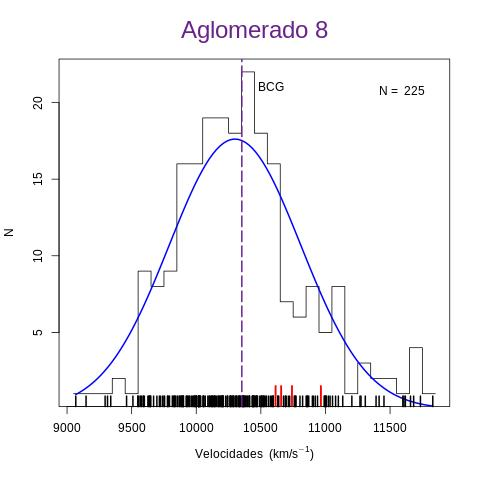
\includegraphics[height=6.7cm,width=9cm]{04-figuras/selec20gap}%
\caption{Histograma Distribuição de Velocidade e Análise de Gaps para o aglomerado 08 do catálogo selec20.}
\textbf{Fonte: Autor.}
\label{fig:selec20gap}%
\end{center}
\end{figure}

O intuito da rotina era identificar a probabilidade de que um \textit{"gap"},  de certo tamanho e em dada localização, possa ser produzido a partir de amostragens aleatórias retiradas de uma gaussiana. As velocidades das galáxias são ordenadas em ordem crescente e o i-ésimo "gap" é definido como $g_i = v_{i+1} - v_i$. O "gap" é ponderado pela sua posição, através de $w_i=i(N-i)$, onde $N$ é o número de galáxias do aglomerado. Os "gaps" ponderados são Não Rejeitados através da divisão por meio da média (MM) da distribuição ordenada do "gap" ponderado dada por: 

\begin{equation}
MM = \frac{2}{N} \sum_{i=N/4}^{3N/4} \sqrt{w_i g_i}
\label{eq:gappomderado}
\end{equation}

Investigamos "gaps" com valores maiores que 2.25, uma vez que em retiradas aleatórias de uma gaussiana, \textit{"gaps"} desse tamanho ocorrem no máximo em 3\% dos casos (vide \citeonline{wainer1978gapping}. \citeonline{beers1991dynamical}). Em seguida os dados foram divididos em duas amostras, contendo objetos com velocidades maiores e velocidades menores que o maior "gap" encontrado, referimos aqui de amostras I e II. Para o caso de aglomerados não encontrado \textit{"gap"} significativo ($>$ 2.25), utilizamos a mediana dos dados como divisor das velocidades do sistema.


A partir de \textit{"gaps"} identificados na distribuição de velocidade, levantou-se o seguinte questionamento: pode eles indicar um gradiente de velocidade em toda distribuição espacial de galáxias? Para isso, estimamos o eixo principal do aglomerado como o resultante do ajuste de uma elipse aos dados projetados no plano do céu, como ilustrado na figura \ref{elipse}. O ajuste foi feito usando-se o pacote \textbf{ellipse} do R.

\begin{figure}[H] %h or !htbp
\vspace{-2pt}
\begin{center}
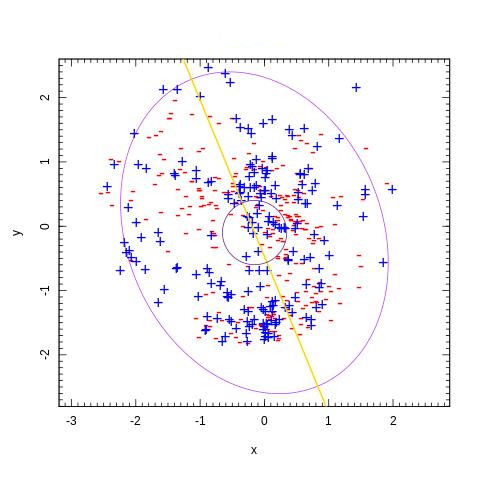
\includegraphics[height=6.7cm,width=9cm]{04-figuras/elipse}%
\caption{Ajuste da elipse e eixo principal da distribuição projetada no plano do céu.}
\textbf{Fonte: Autor.}
\label{elipse}%
\end{center}
\end{figure}


Na Figura \ref{elipse}, vemos o ajuste da elipse na distribuição (X,Y) projetada no plano do céu, com os pontos acima ($+$) e abaixo ($-$) em relação à posição do \textit{gap} principal, indicados em azul e vermelho, respectivamente. A distribuição de galáxias em torno do \textit{gap} de velocidades pode ser utilizada como um indicador indireto da presença ou não de rotação. Estudamos o quanto diferem espacialmente as galáxias de acordo com a sua posição em relação ao eixo principal. Com isso as amostras I e II foram então comparadas em relação a sua distribuição de duas maneiras: independente do eixo principal e em cada lado do eixo. Os testes de comparação de duas amostras utilizados foram o teste de Cramer 2D e o de Hotelling, dos pacotes \textbf{ Cramer} e \textbf{ Hotelling}do R, respectivamente, tendo como a hipótese nula que os pontos $+$ e $-$ foram retirados da mesma população. 

O teste de Cramer para duas amostras pode ser usado para dados univariados e multivariados, como neste trabalho. Para o cálculo do valor crítico uma rotina de \textit{bootstrap} é utilizada e métodos de permutação são usados para obter o valor-p do teste. O teste de Hotelling multivariado compara médias em duas amostras. A rejeição ou não da hipótese nula é feita em todos os casos para um nível de 95\% de confiança. 

Dado que as distribuições espaciais das amostras  I e II sejam distintas com 95\% de confiança em relação aos testes acima citados, interpretamos o resultado como sendo uma indicação indireta de rotação nos aglomerados. Para os aglomerados onde isto acontece, traçamos um perfil de velocidade de rotação ao longo da distância ao centro do aglomerado. A velocidade de rotação foi calculada de maneira cumulativa contra o raio projetado das galáxias de acordo com

\begin{equation}
\omega= \Delta V/R
\label{eq:eq10}
\end{equation}

\noindent onde $\Delta V$ é a diferença de velocidade entre os pontos $+$ e $-$ internos a $R$.

\begin{figure}[H] %h or !htbp
\vspace{-2pt}
\begin{center}
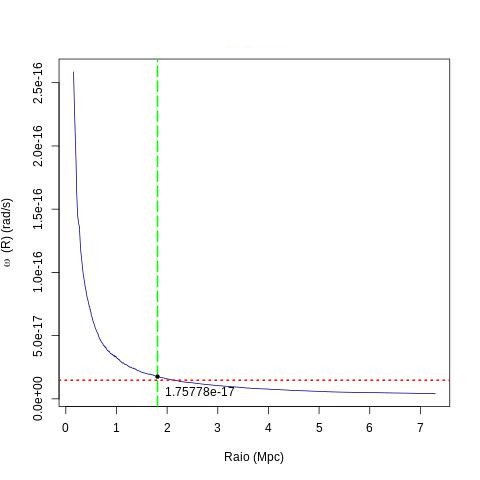
\includegraphics[height=6.7cm,width=9cm]{04-figuras/rotacao}%
\caption{Perfil de velocidade de rotação do aglomerado 08 do catálogo selec20.}
\textbf{Fonte: Autor.}
\label{rotacao}%
\end{center}
\end{figure}

No gráfico a linha tracejada na horizontal refere-se a velocidade de rotação do aglomerado, identificada através do raio (R200) do aglomerado (intersecção da curva de rotação e o valor de R200). Uma vez obtido o valor da velocidade de rotação do aglomerado utilizamos a fórmula dada por \citeonline{lee1969shape} que investigam a dependência da forma e do teorema do virial agindo no movimento orbital. Para que a velocidade angular afete significativamente o cálculo da massa do aglomerado qualquer aceleração centrífuga precisaria ser comparável à aceleração gravitacional. Através da equação \ref{eq:maxRotacao} encontramos o valor limite de detecção de velocidade de rotação do aglomerado, representada na figura \ref{rotacao} pela linha tracejada na vertical.

\begin{equation}
\omega \cong \omega_{orb} = \frac{1}{r^2} \sqrt{G M_g \Delta (1 - e^2)}, 
\label{eq:maxRotacao}
\end{equation}
onde $\omega$ é a velocidade de rotação, G é constante gravitacional, R e M são raio e massa do aglomerado, respectivamente. 

\section{Método de Hwang \& Lee - adaptado}

O método proposto por \citeonline{hwang2007searching}, também usado para identificar a rotação em aglomerados, foi implementado com o propósito de comparar com o nosso método. Eles utilizam a relação sinusoidal para calcular o eixo de rotação ($\Theta_o$) e a velocidade de rotação ($v_{rot}$):

\begin{equation}
 vp(v_{rot}, \Theta) = v_{sys} + v_{rot} . sin(\Theta - \Theta_o) ,
 \label{eq:hwanglee1}
\end{equation}
onde $v_p$ é a velocidade radial de cada galáxia devido a rotação do aglomerado, $v_{sys}$ é a velocidade peculiar do aglomerado e $\Theta$ é o ângulo projetado na posição de cada galáxia no plano céu, partindo do Norte para o Leste. Manolopoulou \&  Plionis, usaram diferenças de velocidade em relação à velocidade média do aglomerado, o valor de $v_{sys}$ foi igual a 0.

O procedimento de minimização do $\chi^2$ foi utilizado para determinar o melhor ajuste dos valores de $v_{rot}$ e $\Theta_0$, representado na equação \ref{hwanglee2}. Ou seja, o conjunto de valores de $v_{rot}$ e $\Theta_0$, são empregados no cálculo de $\chi^2$ para cada par de parâmetros:

\begin{equation}
 \chi^2 (v_{rot}, \Theta_o) = \sum_i{\frac{(v_{pi} - v_{los, i})^2}{\sigma^{2}_{i}}} ,
 \label{hwanglee2}
\end{equation}
onde $v_{los, i}$ é a velocidade de linha de visada de cada galáxia e $\sigma_i$ é a medida em erro.

\chapter{Análise}

Neste trabalho usamos 1000 réplicas dos dados de cada catálogo com intuito de verificar a robustez do método na identificação ou não de rotação. No catálogo I (selec20) 90\% dos casos (18 aglomerados) obtivemos resultados conclusivos, considerando em todas as iterações ou até 900 delas o mesmo resultado, ou seja, a detecção ou não de rotação. Já nos catálogos NoSocs, III sem rotação e III com rotação obtivemos resultados conclusivos em 97.8\% (179 aglomerados), 97\% (194 aglomerados) e 100\% dos casos, respectivamente. Nas seções subsequentes apresentamos os resultados para cada catálogo.     

\section{Catálogo I: selec20}
\textbf{NOSSO MÉTODO}

Os resultados da aplicação de nosso método para o catálogo selec20 são apresentados no Anexo \ref{chap:anexoselec20} e na tabela \ref{tab:selec20T}. Na Figura \ref{selec20gap}, é exibido a análise de \textit{gaps} para um dos 20 aglomerados da amostra, o aglomerado 08. O gráfico na figura contém o histograma da distribuição de velocidades, o ajuste gaussiano superposto (linha em azul), barras inferiores indicando as velocidades individuais ordenadas em ordem crescente , sendo que em vermelho estão indicados os \textit{gaps} com valores maiores que 2.25, ou seja, os \textit{gaps} significativos. Quando mais de um \textit{gap} é encontrado, escolhemos aquele de maior valor; finalmente, a linha vertical tracejada indica a posição da BCG (\textit{brightest cluster galaxy}) apenas como referência. 

\begin{figure}[H] %h or !htbp
\vspace{-2pt}
\begin{center}
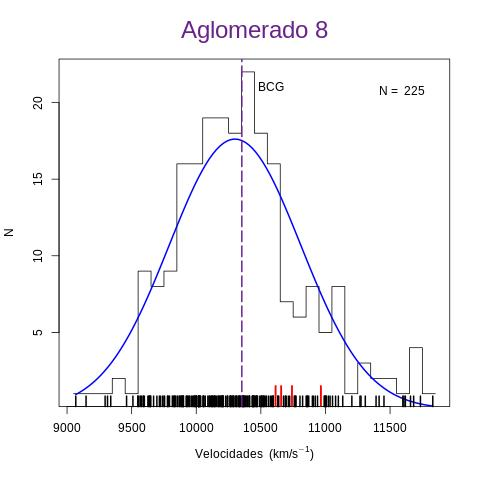
\includegraphics[height=6.7cm,width=9cm]{04-figuras/selec20gap}%
\caption{Histograma Distribuição de Velocidade e Análise de Gaps para o aglomerado 08.}
\textbf{Fonte: Autor.}
\label{selec20gap}%
\end{center}
\end{figure}

Na Figura \ref{selec20ellipse}, vemos o ajuste da elipse na distribuição (X,Y) projetada no plano do céu, com os pontos acima ($+$) e abaixo ($-$) em relação à posição do \textit{gap} principal, indicados em azul e vermelho, respectivamente. A distribuição de galáxias em torno do \textit{gap} de velocidades pode ser utilizada como um indicador indireto da presença ou não de rotação. Estudamos o quanto diferem espacialmente as galáxias de acordo com a sua posição em relação ao eixo principal. A hipótese nula dos testes é a de que os pontos $+$ e $-$ foram retirados da mesma população. Aplicamos dois testes estatísticos, Cramer 2D e Hotelling, em três cenários diferentes: todos os pontos do gráfico, acima e abaixo do eixo principal (Tabela \ref{tab:selec20T}). 

\begin{figure}[H] %h or !htbp
\vspace{-2pt}
\begin{center}
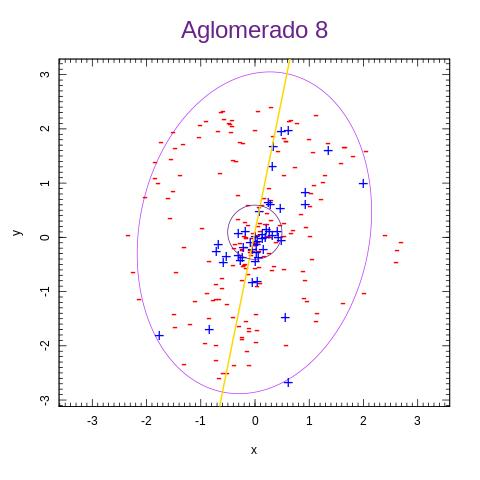
\includegraphics[height=6.7cm,width=9cm]{04-figuras/selec20ellipse}%
\caption{Ajuste da elipse e eixo principal da distribuição projetada no plano do céu para o aglomerado 08.}
\textbf{Fonte: Autor.}
\label{selec20ellipse}%
\end{center}
\end{figure}

\begin{table}[H]
\caption{Teste Cramer e Hotelling aplicado no catálogo selec20.}
\vspace{12pt}
\centering{}
\resizebox{1.0\textwidth}{!}{
\begin{tabular}{llllllll}
\hline
\multirow{2}{*}{\textbf{Cluster}}  & \multicolumn{2}{|c|}{\textbf{Cenário 1}} & \multicolumn{2}{c|}{\textbf{Cenário 2}} & \multicolumn{2}{c|}{\textbf{Cenário 3}} & \multirow{2}{*}{\textbf{Nº galáxias}} \\ \cline{2-7}
                         & \textbf{Cramer}       & \textbf{Hotelling}       & \textbf{Cramer}       & \textbf{Hotelling}       & \textbf{Cramer}       & \textbf{Hotelling}       &                              \\ \hline
01  &  0.496503 & 0.616007 & 0.768232 &  0.871778 & 0.364635 & 0.746935 & 223 \\ 
02  &  {\color{red}0.003996} & {\color{red}0.007875} &  0.076923 &  0.006919 & {\color{red}0.021978} & {\color{red}0.091680} & 244 \\ 
03  &  0.298701 & 0.561228 &  0.648352 &  0.202482 & 0.060939 & 0.129923 & 177 \\   
04  &  {\color{red}0}  & {\color{red}9.769963e-15} & {\color{red}0} &  2.334383e-07 & {\color{red}0.006993007} & {\color{red}0.01569305} & 435 \\ 
05  &  0.097902 & {\color{red}0.048305} & {\color{red}0.044955} & 0.072319 & 0.082917 & 0.396323 & 951\\ 
06  &  0.281718 & 0.265025 &  0.472528 &  0.804144 & 0.257742 & 0.414097 & 165 \\ 
07  &  {\color{red}0.041958} & 0.588022 & 0.556444 &  0.634652 & {\color{red}0.038961} & 0.884234 & 313 \\ 
08  &  {\color{red}0.009990} & 0.444646 & {\color{red}0.011988} & 0.080753 & 0.071928 & 0.055154 & 225 \\ 
09  &  {\color{red}0.028971} & 0.230194 & {\color{red}0.035964} & {\color{red}0.037384} & 0.095904 & {\color{red}0.036469} & 215 \\ 
10  &  {\color{red}0.000999} & {\color{red}0.006792} &  {\color{red}0.003996} & {\color{red}0.025815} & 0.502498 & 0.803647 & 308 \\ 
11  &  {\color{red}0.000999} & {\color{red}0.003167} &  0.335664 &  0.900630 & {\color{red}0.000999} & 0.069658 & 651 \\ 
12  &  {\color{red}0}  & {\color{red}1.130531e-10} & {\color{red}0} &   3.967377e-05 &  {\color{red}0} &  1.773186e-07 &  173 \\ 
13  &  0.106893 & 0.698218 &  0.133866 &  0.151622 & 0.265734 & 0.332495 & 218 \\ 
14  &  {\color{red}0.038961} & 0.005413 & 0.475525 &  0.211045 & 0.760240 & 0.501961 & 127 \\ 
15  &  0.117882 & 0.574480 &  0.341658 &  0.224218 & {\color{red}0.036963} & 0.060953 & 114 \\ 
16  &  {\color{red}0.044955} & 0.518194 & {\color{red}0.002997} &  {\color{red}0.019457} & 0.408591 & 0.477522 & 144  \\ 
17  &  {\color{red}0}  & {\color{red}2.202682e-13} & {\color{red}0} &  3.47107e-05 & 0.2367632 & 0.3371383 & 773 \\ 
18  &  {\color{red}0} & {\color{red}0.04275908} & {\color{red}0.01498501} &  {\color{red}0.007541272} & 0.1298701 & 0.753498 & 233 \\ 
19  &  0.087912 & 0.406300 &  0.299700 &  0.295311 & 0.137862 & 0.239693 & 113 \\ 
20  &  0.118881 & 0.903751 &  0.072927 &  0.317330 & 0.128871 & 0.229752 & 210 \\ \hline
\label{tab:selec20T}
\end{tabular}
}
\end{table}

O teste de Cramer para duas amostras pode ser usado para dados univariados e multivariados, como neste trabalho. Para o cálculo do valor crítico uma rotina de \textit{bootstrap}é utilizada e métodos de permutação são usados para obter o valor-p do teste. O teste de Hotelling multivariado compara médias em duas amostras. A rejeição ou não da hipótese nula é feita em todos os casos para um nível de 95\% de confiança. 

Consideramos evidência significativa de rotação se houve rejeição da hipótese nula em pelo menos um dos cenários testadas. Isto nos leva a 14 aglomerados com evidência de algum grau de rotação. São eles os aglomerados: 02, 04, 05, 07, 08, 09, 10, 11, 12, 14, 15, 16, 17 e 18. Em uma análise mais criteriosa verificamos que:

\begin{itemize}
   	\item 28.57\% dos aglomerados houve rejeição da hipótese nula (indicando rotação) em pelo menos um dos testes (Cramer e Hotelling) nos três cenários (todos os pontos, acima e abaixo do eixo principal). 
   	\item 42.86\% dos aglomerados houve rejeição da hipótese nula em pelo menos um dos testes em dois cenários.
   	\item 7.14\% dos aglomerados houve rejeição da hipótese nula nos dois testes em apenas um cenário.
   	\item 7.14\% dos aglomerados houve rejeição da hipótese nula em pelo menos um dos testes em apenas um cenário.
 \end{itemize} 

Finalmente, calculamos o perfil de velocidade de rotação para estes quatorze aglomerados, como ilustrado na Figura \ref{selec20rotacao}. A velocidade de rotação foi calculada de maneira cumulativa contra o raio projetado das galáxias de acordo com

\begin{equation}
\omega= \Delta V/R
\label{eq:eq10}
\end{equation}

\noindent onde $\Delta V$ é a diferença de velocidade entre os pontos $+$ e $-$ internos a $R$.

\begin{figure}[H] %h or !htbp
\vspace{-2pt}
\begin{center}
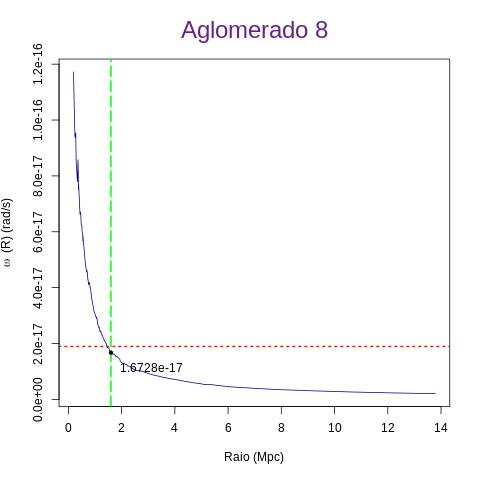
\includegraphics[height=6.7cm,width=9cm]{04-figuras/selec20rotacao}%
\caption{Perfil de velocidade de rotação para o aglomerado 08.}
\textbf{Fonte: Autor.}
\label{selec20rotacao}%
\end{center}
\end{figure}

No gráfico o valor exibido é a velocidade de rotação do aglomerado determinado a partir do R200 e a linha na vertical, o valor em y, é a velocidade limite para detecção de rotação no aglomerado, calculado pela fórmula da equação \ref{eq:maxRotacao}. 

\textbf{MÉTODO DE HWANG \& LEE}

Aplicamos o método de Hwang \& Lee para o catálogo selec20 e os resultados são apresentados na tabela \ref{tab:selec20hwang}. Para todos os aglomerados foi detectado um grau de rotação.

 \begin{table}[H]
\caption{Resultado do métdo Hwang \& Lee para o catálogo selec20.}
\vspace{12pt}
\centering{}
\resizebox{.8\textwidth}{!}{
\begin{tabular}{ccccc}
\cline{1-4}
\textbf{Cluster} & \textbf{Velocidade Rotacional} & \textbf{Ângulo (radiano)} & \textbf{Ângulo (grau)} \\ \hline
1 & -724.22 & 2.30 & 132.16 \\ 
2 & -661.24 & 2.71 & 155.55 \\ 
3 & -1016.65 & 1.76 & 101.24 \\ 
4 & 750.69 & 2.09 & 119.86 \\ 
5 & -790.08 & 1.19 & 68.58 \\ 
6 & 656.37 & 0.78 & 44.99 \\ 
7 & -1067.90 & 2.63 & 151.15 \\ 
8 & 852.35 & 0.14 & 8.03 \\ 
9 & 703.58 & 2.18 & 125.32 \\ 
10 & -873.78 & 1.67 & 96.15 \\ 
11 & -1117.95 & 2.80 & 160.61 \\ 
12 & -946.77 & 3.06 & 175.81 \\ 
13 & -891.43 & 2.46 & 141.01 \\ 
14 & -625.88 & 0.47 & 27.14 \\ 
15 & 864.45 & 0.27 & 15.92 \\ 
16 & -1041.45 & 1.01 & 57.90 \\ 
17 & -505.15 & 2.55 & 146.42 \\ 
18 & 889.73 & 0.81 & 46.55 \\ 
19 & -1062.70 & 3.02 & 173.57 \\ 
20 & 944.22 & 1.90 & 109.37 \\ \hline
\end{tabular}
}
\label{tab:selec20hwang}
\end{table}


\section{Catálogo II: NoSOCS}
\textbf{NOSSO MÉTODO}

No catálogo de NoSOCS, diferente do selec20, 56.33\% dos aglomerados (um total de 89) não apresentaram \textit{gaps} significativos, nestes casos os dados foram divididos pelo cálculo da mediana. Além disso, 13.66\%, cerca de 25 aglomerados, continham um total inferior a 20 objetos, o que tornava o cálculo de detecção de rotação inviável. Por esse motivo, reduzimos a amostra de 183 para 158 aglomerados.

Aplicamos os mesmos cenários e testes usados no catálogo selec20 e verificamos que:

\begin{itemize}
   	\item 34.43\% dos aglomerados apresentaram indicação direta de rotação, levando em conta um dos testes (Cramer e Hotelling) em pelo menos um cenário. Considerando-se que 47.62\% apenas as amostras sem \textit{gap}, ou seja, em casos onde os dados foram divididos pela mediana. 
   	\item Desse total, tendo em conta a rejeição da hipótese em ambos os testes para os três cenários um total de 6.35\%, dois cenários 15.87\% e um cenário 9.52\%.
   	\item Já a rejeição da hipótese em pelo menos um dos testes para os três cenários um total de 11.11\%, dois cenários 15.87\% e um cenário 41.27\%. 
 \end{itemize} 

 Os resultados são apresentados nas tabelas \ref{tab:nosocsI} e \ref{tab:nosocsII} e no Anexo \ref{chap:anexonosocs}. 

\begin{table}[H]
\caption{Teste Cramer e Hotelling aplicado no catálogo NoSOCS com rotação detectada utilizando gap.}
\vspace{12pt}
\centering{}
\resizebox{.9\textwidth}{!}{
\begin{tabular}{cccccccc}
\hline
\multirow{2}{*}{\textbf{Cluster}} & \multicolumn{2}{|c|}{\textbf{Cenário 1}} & \multicolumn{2}{c|}{\textbf{Cenário 2}} & \multicolumn{2}{c|}{\textbf{Cenário 3}} & \multirow{2}{*}{\textbf{Nº galáxias}} \\ \cline{2-7}
                         & \multicolumn{1}{|c}{\textbf{Cramer}}       & \textbf{Hotelling}       & \textbf{Cramer}       & \textbf{Hotelling}       & \textbf{Cramer}       & \textbf{Hotelling}                                  \\ \hline
01238 & {\color{red}0.003996}	& {\color{red}0.005606} & {\color{red}0.021978} & {\color{red}0.025209} & 0.056943 & 0.150563 & 44 \\ 
01836 & 0 & 0.000395 & 0.006993 & 0.010808 &  0.022977 & 0.001210 & 86 \\ 
02440 & {\color{red}0.017982} & {\color{red}0.090600} & {\color{red}0.069930} & {\color{red}0.005757} & {\color{red}0.150849} & {\color{red}0.137841} & 41 \\ 
02447 & 0.511488 & 0.646515 & {\color{red}0.031968} & 0.053283 & 0.743256 & 0.548081 & 46 \\ 
04681 & {\color{red}0.014985} & {\color{red}0.017471} & {\color{red}0.024975} & {\color{red}0.047805} & 0.204795 & 0.212804 & 162 \\ 
04703 & {\color{red}0.001998} & {\color{red}0.000551} & {\color{red}0.027972} & {\color{red}0.018654} & 0.109890 & 0.149901 & 91 \\ 
06256 & {\color{red}0.035964} & {\color{red}0.016620} & {\color{red}0.026973} & {\color{red}0.013306} & 0.283716 & 0.368284 & 37 \\ 
06547 & {\color{red}0} & {\color{red}0.005209} & 0.562437 & 0.849069 & {\color{red}0.001998} & {\color{red}0.005002} & 112 \\ 
07217 & 0.077922 & {\color{red}0.038481} & 0.382617 & 0.433854 & 0.152847 & 0.456518 & 24 \\ 
07703 & {\color{red}0.043956} & 0.079676 & {\color{red}0.005994} & {\color{red}0.015114} & 0.586413 & 0.980806 & 48 \\ 
09148 & {\color{red}0.012987} & {\color{red}0.004465} & {\color{red}0.048951} & 0.112433 & {\color{red}0.022977} & 0.089178 & 31 \\ 
10008 & {\color{red}0.001998} & 0.293476 & {\color{red}0.029970} & 0.387069 & {\color{red}0.025974} & 0.143509 & 123 \\ 
10013 & {\color{red}0.008991} & {\color{red}0.031328} & 0.287712 & 0.832952 & 0.377622 & 0.582334 & 86 \\ 
10015 & {\color{red}0.003996} & 0.057669 & 0.092907 & 0.279563 & {\color{red}0.029970} & 0.057429 & 139 \\ 
10020 & {\color{red}0.000999} & {\color{red}0.008616} & {\color{red}0.003996} & 0.403677 & {\color{red}0.004995} & {\color{red}0.016639} & 114 \\ 
10021 & {\color{red}0.004995} & {\color{red}0.030595} & {\color{red}0.012987} & {\color{red}0.015253} & NA & NA & 89 \\ 
10023 & {\color{red}0.040959} & 0.084825 & 0.078921 & 0.277558 & 0.110889 & 0.277176 & 107 \\ 
10024 & {\color{red}0.037962} & 0.074983 & 0.090909 & 0.255343 & 0.231768 & 0.413339 & 113 \\ 
10027 & 0.163836 & 0.413906 & 0.268731 & 0.393231 & {\color{red}0.035964} & 0.059391 & 86 \\ 
10029 & {\color{red}0.025974} & 0.056490 & {\color{red}0.048951} & 0.165669 & 0.057942 & 0.058164 & 135 \\ 
10030 & {\color{red}0} & 3.06E+01 & {\color{red}0.013986} & {\color{red}0.015258} & {\color{red}0} & 5.74E+01 & 87 \\ 
10037 & {\color{red}0.000999} & {\color{red}0.008946} & {\color{red}0.032967} & 0.285959 & 0.070929 & 0.157548 & 145 \\ 
10043 & {\color{red}0.020979} & 0.059925 & 0.053946 & 0.061660 & 0.188811 & 0.271167 & 218 \\ 
10044 & {\color{red}0} & 1.10E+01 & {\color{red}0.003996} & {\color{red}0.008143} & {\color{red}0.001998} & {\color{red}0.001075} & 177 \\ 
10045 & 0.103896 & 0.281427 & {\color{red}0.037962} & 0.093578 & 0.481518 & 0.961108 & 55 \\ 
10051 & {\color{red}0.045954} & 0.240987 & {\color{red}0} & {\color{red}0.003778} & 0.214785 & 0.067199 & 189 \\ 
10053 & 0.065934 & 0.559379 & {\color{red}0} & {\color{red}0.000141} & {\color{red}0.001998} & {\color{red}0.001089} & 447 \\ 
10054 & {\color{red}0} & {\color{red}0.006898} & 0.201798 & 0.576037 & {\color{red}0} & {\color{red}0.010700} & 537 \\ 
10056 & {\color{red}0.025974} & {\color{red}0.020923} & 0.160839 & {\color{red}0.047179} & 0.318681 & 0.373086 & 100 \\ 
10059 & {\color{red}0.041958} & 0.424066 & 0.111888 & 0.290470 & 0.309690 & 0.404923 & 150 \\ 
10060 & 0.201798 & 0.917590 & {\color{red}0.005994} & {\color{red}0.048580} & 0.831168 & 0.647436 & 133 \\ 
10063 & 0.099900 & 0.695755 & {\color{red}0.049950} & 0.189107 & {\color{red}0.033966} & 0.102787 & 219 \\ 
10064 & 0.096903 & {\color{red}0.042881} & 0.279720 & 0.139438 & 0.628371 & 0.789767 & 133 \\ \hline
\label{tab:nosocsI}
\end{tabular}
}
\end{table}

\begin{table}[H]
\caption{Teste Cramer e Hotelling aplicado no catálogo NoSOCS com rotação detectada utilizando mediana.}
\vspace{12pt}
\centering{}
\resizebox{.9\textwidth}{!}{
\begin{tabular}{cccccccc}
\hline
\multirow{2}{*}{\textbf{Cluster}} & \multicolumn{2}{|c|}{\textbf{Cenário 1}} & \multicolumn{2}{c|}{\textbf{Cenário 2}} & \multicolumn{2}{c|}{\textbf{Cenário 3}} & \multirow{2}{*}{\textbf{Nº galáxias}} \\ \cline{2-7}
                         & \multicolumn{1}{|c}{\textbf{Cramer}}       & \textbf{Hotelling}       & \textbf{Cramer}       & \textbf{Hotelling}       & \textbf{Cramer}       & \textbf{Hotelling}       &                              \\ \hline
01831 & {\color{red}0} & {\color{red}0.002671} & {\color{red}0.001998} & {\color{red}0.031291} & {\color{red}0.009990} & {\color{red}0.004074} & 72 \\
02137 & {\color{red}0.036963} & 0.347093 & 0.248751 & 0.329532 & 0.161838 & 0.732693 & 34 \\
02433 & 0.118881 & 0.301255 & 0.846153 & NA & {\color{red}0.032967} & 0.216530 & 31 \\
03176 & {\color{red}0.040959} & 0.437995 & 0.155844 & 0.161899 & 0.111888 & 0.723103 & 26 \\
03691 & 0.060939 & {\color{red}0.031896} & 0.464535 & 0.534411 & 0.435564 & 0.115439 & 43 \\
03907 & 0.114885 & 0.168692 & {\color{red}0.015984} & 0.065279 & 0.606393 & 0.998517 & 44 \\
04048 & 0.139860 & {\color{red}0.023276} & 0.252747 & 0.213522 & 0.817182 & 0.59885 & 30 \\
04409 & {\color{red}0.000999} & {\color{red}0.001251} & 0.101898 & 0.178182 & {\color{red}0.006993} & {\color{red}0.01041} & 23 \\
04470 & {\color{red}0.047952} & 0.110327 & 0.511488 & NA & 0.056943 & 0.136180 & 35 \\
04479 & 0.090909 & 0.173748 & 0.830169 & 0.069908 & {\color{red}0.013986} & {\color{red}0.020507} & 25 \\
04672 & 0.354645 & 0.600566 & 0.540459 & 0.433777 & 0.168831 & {\color{red}0.024215} & 48 \\
05359 & 0.096903 & 0.116698 & {\color{red}0.010989} & {\color{red}0.025032} & 0.483516 & 0.702417 & 62 \\
05447 & {\color{red}0}        & {\color{red}0.001094} & {\color{red}0.023976} & {\color{red}0.046308} & {\color{red}0.007992} & {\color{red}0.015626} & 57 \\
06207 & 0.626373 & 0.378981 & 0.268231 & {\color{red}0.007777} & 0.709290 & 0.595039 & 21 \\
06286 & 0.129870 & 0.054084 & {\color{red}0.019980} & {\color{red}0.013322} & 0.130869 & 0.159239 & 70 \\
07395 & 0.328671 & 0.777906 & 0.409590 & 0.673840 & 0.136863 & {\color{red}0.000785} & 29 \\
08022 & 0.266733 & 0.857210 & {\color{red}0.040959} & 0.259307 & 0.147852 & 0.150297 & 51 \\
08721 & {\color{red}0.032967} & 0.129166 & 0.225774 & 0.515822 & 0.084915 & 0.275898 & 47 \\
09061 & 0.302697 & {\color{red}0.037116} & 0.805194 & 0.896726 & 0.517482 & 0.067197 & 46 \\
10006 & {\color{red}0.040959} & 0.084762 & 0.195804 & 0.602401 & {\color{red}0.018981} & {\color{red}0.005725} & 74 \\
10016 & {\color{red}0.000999} & {\color{red}0.000896} & {\color{red}0.034965} & 0.072791 & {\color{red}0.000999} & {\color{red}0.005635} & 92 \\
10018 & 0.398601 & 0.331314 & {\color{red}0.047952} & 0.807257 & 0.330669 & 0.141546 & 65 \\
10026 & {\color{red}0.033966} & {\color{red}0.036372} & 0.531468 & 0.680673 & {\color{red}0}        & {\color{red}0.001887} & 130 \\
10028 & {\color{red}0.018981} & {\color{red}0.018787} & 0.231768 & 0.274238 & 0.053946 & 0.052530 & 80 \\
10031 & {\color{red}0}        & {\color{red}6.43E-03} & {\color{red}0.002997} & {\color{red}0.001092} & {\color{red}0}        & {\color{red}1.80E-04} & 141 \\
10035 & 0.122877 & 0.156720 & 0.505494 & 0.996701 & {\color{red}0.029970} & 0.074546 & 58 \\
10036 & 0.410589 & 0.917501 & 0.056943 & {\color{red}0.045570} & 0.670329 & 0.544576 & 119 \\
10040 & {\color{red}0.000999} & {\color{red}0.001944} & {\color{red}0.036963} & 0.059351 & {\color{red}0.007992} & {\color{red}0.009938} & 99 \\
10050 & {\color{red}0.020979} & 0.595124 & 0.068931 & 0.279501 & 0.077922 & 0.050991 & 77 \\
10055 & {\color{red}0}        & 0.362105 & 0.260739 & 0.180886 & {\color{red}0}        & {\color{red}0.000790} & 104 \\ \hline

\label{tab:nosocsII}
\end{tabular}
}
\end{table}

\textbf{MÉTODO DE HWANG \& LEE}

Aplicamos o método de Hwang \& Lee para o catálogo NoSocs e os resultados são apresentados na tabela \ref{tab:nosocshwang}. Cerca de 97.81\% dos aglomerados (179) detectaram rotação. Apenas os aglomerados 02907, 04537, 04537 e 10046 não identificaram grau de rotação.

{\small
\begin{longtable}{ccccc}
\caption{Resultado do métdo Hwang \& Lee para o catálogo NoSocs.}\label{tab:nosocshwang}
\\ \hline
\textbf{Cluster} & \textbf{Velocidade Rotacional} & \textbf{Ângulo (radiano)} & \textbf{Ângulo (grau)} \\ \hline
00053 & -587.01 & 3.14159265358979 & 179.981843124159 \\
00086 & 53.72 & 0 & 0 \\
00339 & -1184.3 & 3.04492826424857 & 174.4439402588 \\
00719 & 488.11 & 0.826734908839419 & 47.3636429274103 \\
00996 & 969.01 & 0.966643893412244 & 55.3790286535875 \\
01052 & 328.83 & 1.80879577024867 & 103.625909677546 \\
01189 & -660.52 & 2.73882436466802 & 156.907247851831 \\
01238 & -550.9 & 0.14612058853906 & 8.37124851740276 \\
01264 & 782.77 & 0.628318530717959 & 35.9963686248319 \\
01347 & 644.07 & 3.14159265358979 & 179.981843124159 \\
01478 & 801.69 & 0.589048622548086 & 33.7465955857799 \\
01831 & -1184.3 & 1.68141578642834 & 96.3283104044796 \\
01836 & -356.53 & 2.36543446858526 & 135.515740705249 \\
01877 & 665.09 & 1.86168453546062 & 106.655907036539 \\
01933 & 643.25 & 2.20319484797206 & 126.221032840319 \\
02035 & -383.23 & 1.47839654286579 & 84.6973379407808 \\
02104 & 940.53 & 2.33948389097112 & 134.029032113736 \\
02137 & 1016.62 & 1.71359599286716 & 98.1719144313596 \\
02182 & 581.02 & 0.872664625997165 & 49.9949564233776 \\
02186 & 631.46 & 2.51327412287183 & 143.985474499327 \\
02249 & 1085.4 & 1.25663706143592 & 71.9927372496637 \\
02298 & 761.16 & 0.336599212884621 & 19.2837689061599 \\
02301 & -816.24 & 2.25005960324674 & 128.905914670006 \\
02433 & -352.08 & 1.25663706143592 & 71.9927372496637 \\
02440 & -503.39 & 0.392699081698724 & 22.4977303905199 \\
02447 & 631.46 & 0.907571211037051 & 51.9947546803127 \\
02469 & -1002.72 & 0.628318530717959 & 35.9963686248319 \\
02490 & 789.35 & 1.91227378914161 & 109.554165379923 \\
02752 & 177.52 & 2.26194671058465 & 129.586927049395 \\
02759 & 672.73 & 1.14239732857811 & 65.4479429542397 \\
02789 & 376.12 & 0.196349540849362 & 11.24886519526 \\
02827 & -116.21 & 0.369599135716446 & 21.1743344851952 \\
02899 & -286.98 & 2.1918088280859 & 125.568727761041 \\
02907 & - & - &  -  \\
03031 & -771.63 & 3.14159265358979 & 179.981843124159 \\
03112 & 561.62 & 0.966643893412244 & 55.3790286535875 \\
03176 & 722.25 & 0.628318530717959 & 35.9963686248319 \\
03229 & 436.91 & 0.538558740615393 & 30.8540302498559 \\
03459 & -1042.44 & 2.0616701789183 & 118.11308455023 \\
03565 & -404.09 & 0.490873852123405 & 28.1221629881499 \\
03631 & -1184.3 & 2.79252680319093 & 159.983860554808 \\
03691 & -751.98 & 0.299199300341885 & 17.1411279165866 \\
03742 & -842.29 & 0.387319642223399 & 22.1895423029785 \\
03898 & -1184.3 & 0.649984686949612 & 37.2376227153433 \\
03907 & -603.68 & 0.21918088280859 & 12.5568727761041 \\
03915 & -324.57 & 1.0471975511966 & 59.9939477080531 \\
03975 & -191.31 & 0.883572933822129 & 50.6198933786698 \\
04023 & -715.56 & 2.90255842994709 & 166.287572451669 \\
04048 & 1007.13 & 1.7332924985323 & 99.3003272409155 \\
04100 & 517.97 & 1.65806278939461 & 94.9904172044174 \\
04376 & 761.16 & 1.90739553967952 & 109.27469046824 \\
04404 & 672.73 & 2.85599332144527 & 163.619857385599 \\
04405 & 217.57 & 0.0923997839291116 & 5.2935836212988 \\
04409 & -977.96 & 2.14199499108395 & 122.714893039199 \\
04458 & 594.65 & 1.10380282423425 & 63.2368638003803 \\
04470 & -316.47 & 2.4023943821569 & 137.633174153769 \\
04479 & -238.59 & 1.96349540849362 & 112.4886519526 \\
04537 & -276.42 & 0 & 0 \\
04641 & 328.83 & 1.25663706143592 & 71.9927372496637 \\
04672 & -942.84 & 3.00790785982001 & 172.323041289089 \\
04681 & 958.52 & 0.468311948361211 & 26.8295915216138 \\
04703 & 1034.96 & 1.78023583703422 & 101.98971110369 \\
04710 & 599.04 & 2.80499344070517 & 160.698074217999 \\
05039 & -860.06 & 0.448798950512828 & 25.7116918748799 \\
05206 & 177.52 & 1.63362817986669 & 93.5905584245628 \\
05325 & -690.89 & 2.86841068371242 & 164.331248069885 \\
05359 & -700.59 & 2.00855923754102 & 115.070358718725 \\
05447 & 315.32 & 0.504898819326931 & 28.9256533592399 \\
05535 & -522.3 & 1.30899693899575 & 74.9924346350663 \\
05717 & 916.02 & 1.8286882610448 & 104.765550475257 \\
05780 & 1085.4 & 0 & 0 \\
05859 & 768.7 & 0.949783825503891 & 54.4131153631179 \\
05908 & -745 & 0.405366794011586 & 23.2234636289238 \\
06070 & 653.08 & 0.673198425769241 & 38.5675378123198 \\
06173 & -1184.3 & 1.2875379727827 & 73.763050460721 \\
06175 & -276.42 & 2.82743338823081 & 161.983658811743 \\
06184 & -1016.17 & 2.21075038585948 & 126.65388960589 \\
06207 & -616.88 & 3.14159265358979 & 179.981843124159 \\
06233 & 697.89 & 0.996114743821154 & 57.0674136735139 \\
06256 & -679.92 & 0.698131700797732 & 39.9959651387021 \\
06261 & -1184.3 & 1.67105992212223 & 95.7350229383826 \\
06264 & -197.47 & 1.77568280420293 & 101.728867852786 \\
06286 & -625.1 & 3.050531996964 & 174.764978106068 \\
06392 & -377.3 & 1.18682389135614 & 67.9931407357935 \\
06447 & 457.61 & 1.80474471589201 & 103.393824773453 \\
06475 & -739.26 & 1.10879740714934 & 63.5230034555856 \\
06506 & 1039.08 & 1.21816857996339 & 69.7888779461026 \\
06508 & -639.57 & 2.01061929829747 & 115.188379599462 \\
06547 & 942.27 & 1.69815819112962 & 97.2874827698158 \\
06723 & -427.73 & 1.49599650170943 & 85.705639582933 \\
06758 & -697.94 & 2.91719317833338 & 167.125997186719 \\
06841 & 678.02 & 2.98048533802109 & 170.752005015228 \\
06861 & -616.88 & 0.392699081698724 & 22.4977303905199 \\
06924 & -922.41 & 1.32913535344184 & 76.1461643986828 \\
07204 & -771.63 & 0.999597662505843 & 57.2669500849598 \\
07217 & 98.57 & 2.45863772889636 & 140.855355488472 \\
07395 & 274.79 & 1.90739553967952 & 109.27469046824 \\
07435 & -907.51 & 0.383121055315828 & 21.9490052590438 \\
07520 & -427.73 & 3.14159265358979 & 179.981843124159 \\
07584 & 1085.4 & 2.79252680319093 & 159.983860554808 \\
07703 & -797.97 & 2.87422306605024 & 164.664239454018 \\
07775 & 917.27 & 2.90888208665722 & 166.649854744592 \\
07815 & 561.62 & 1.93328778682449 & 110.758057307175 \\
07837 & 653.08 & 2.54319405290602 & 145.699587290986 \\
07975 & -1119.45 & 0.448798950512828 & 25.7116918748799 \\
08022 & 722.25 & 1.63362817986669 & 93.5905584245628 \\
08049 & - & - &  -  \\
08173 & 1085.4 & 2.73181969877373 & 156.505950542747 \\
08219 & 722.25 & 0.879645943005142 & 50.3949160747646 \\
08291 & -914.1 & 0.747998250854713 & 42.8528197914665 \\
08338 & 684.86 & 3.14159265358979 & 179.981843124159 \\
08710 & -1039.43 & 1.06947835015823 & 61.2704146805648 \\
08720 & - & - &  -  \\
08721 & -1184.3 & 2.5269332213657 & 144.768004252041 \\
08738 & -911.94 & 2.95309709437441 & 169.18293253671 \\
08742 & -896.08 & 2.69279370307697 & 154.270151249279 \\
08975 & 740.01 & 0.478068447285403 & 27.3885413449808 \\
09061 & -1133.86 & 1.60570291183478 & 91.9907198190147 \\
09075 & -706.47 & 2.97624567182191 & 170.509114538677 \\
09132 & -394.84 & 3.14159265358979 & 179.981843124159 \\
09144 & - & - & - \\
09148 & -427.73 & 2.0943951023932 & 119.987895416106 \\
09153 & 789.35 & 0.956136894570807 & 54.7770826899615 \\
09157 & 490.95 & 3.06679282850432 & 175.696561145013 \\
09162 & 431.42 & 1.8636566589092 & 106.768889988908 \\
09176 & 730.76 & 1.99622033196851 & 114.363462818476 \\
09177 & 156.89 & 2.85599332144527 & 163.619857385599 \\
10001 & 362.21 & 0.554398703574669 & 31.7615017277928 \\
10004 & -863.87 & 0.702238357861248 & 40.2312355218709 \\
10006 & 525.75 & 1.506243053091 & 86.2926645115832 \\
10008 & -1128.49 & 0.283258354012194 & 16.2278711013586 \\
10009 & -849.43 & 2.21456531318625 & 126.87244679244 \\
10010 & -659.22 & 2.32102740824918 & 132.971660218595 \\
10013 & -650.25 & 2.21759481429868 & 127.046006911171 \\
10014 & 1085.4 & 2.64555170828614 & 151.563657367713 \\
10015 & 509.75 & 0.61465943222409 & 35.2138388721181 \\
10016 & 786.1 & 0.138091984773178 & 7.91128980765535 \\
10017 & -1053.86 & 2.05828484200711 & 117.919138598587 \\
10018 & -1077.91 & 1.17809724509617 & 67.4931911715597 \\
10019 & -1071.62 & 0.445615979232595 & 25.5293394502354 \\
10020 & -441.12 & 0.500430688182445 & 28.6696741259723 \\
10021 & 1085.4 & 1.21379716161424 & 69.5384393888797 \\
10022 & 780.93 & 1.1110510604159 & 63.6521152512271 \\
10023 & -841.7 & 1.7189846595114 & 98.4806311434079 \\
10024 & -1042.44 & 2.04764521171478 & 117.309594179139 \\
10025 & -1020.88 & 3.06619442990364 & 175.662278889179 \\
10026 & 839.08 & 3.06853235932026 & 175.796218865458 \\
10027 & 978.59 & 0.0369599135716446 & 2.11743344851952 \\
10028 & -695.88 & 0.119300986845182 & 6.83475353636048 \\
10029 & 1034.59 & 3.07125848970345 & 175.952398875111 \\
10030 & -392.54 & 1.49773603252537 & 85.8052973033783 \\
10031 & 890.85 & 1.12199737628207 & 64.2792296871997 \\
10032 & -271.49 & 1.43420534185621 & 82.1656240349423 \\
10033 & 537.54 & 0.361102603860896 & 20.6875681751907 \\
10034 & 601.69 & 0.772522783669621 & 44.2578302764326 \\
10035 & 926.12 & 0.936966230018008 & 53.6787953177317 \\
10036 & -1165.07 & 2.95522698769887 & 169.304954125268 \\
10037 & -679.92 & 3.05432619099008 & 174.982347481822 \\
10038 & 615.34 & 0.111535833855259 & 6.38988792156778 \\
10039 & 626.06 & 1.0471975511966 & 59.9939477080531 \\
10040 & 575.88 & 0.160285339468867 & 9.18274709817139 \\
10041 & -1042.44 & 3.14159265358979 & 179.981843124159 \\
10042 & -305.71 & 1.82415057305214 & 104.505586330157 \\
10043 & 196.35 & 2.57697461907365 & 147.63487592673 \\
10044 & 995.13 & 1.05314753728294 & 60.3348224109397 \\
10045 & 1043.37 & 1.51261868506175 & 86.6579244671878 \\
10046 & - & - &  -  \\
10047 & -782.58 & 1.61249888414343 & 92.3800610725773 \\
10048 & -1158.99 & 0.992696563401979 & 56.8715861172994 \\
10049 & -383.23 & 1.15499729911389 & 66.169795266235 \\
10050 & -587.01 & 1.24010236325913 & 71.0454643911155 \\
10051 & 409.32 & 2.57343228006823 & 147.431935325109 \\
10052 & -276.42 & 0.773315114729795 & 44.30322292287 \\
10053 & 1003.98 & 1.3876541541641 & 79.4987064920614 \\
10054 & -629.58 & 2.58478052282295 & 148.082076152527 \\
10055 & -875.8 & 0.33550989504357 & 19.2213618870461 \\
10056 & -1092.59 & 1.87226228850301 & 107.261906508337 \\
10058 & -902.06 & 0.0162776821429523 & 0.932548409969737 \\
10059 & -194.16 & 2.46688819107386 & 141.328024466622 \\
10060 & 793.09 & 2.21339482412008 & 126.805389473839 \\
10062 & -906.38 & 1.66696753047622 & 95.5005698209824 \\
10063 & 398.24 & 2.81014021766059 & 160.992933069775 \\
10064 & 414.81 & 1.28519699465037 & 73.6289358235197 \\ \hline
\end{longtable}
}

\section{Catálogo III: }
\textbf{NOSSO MÉTODO}

Utilizamos o método descrito na seção \ref{subsec:simulate} na geração de duas amostras, com e sem rotação, que chamaremos de amostra I e II, respectivamente, cada uma com 200 elementos. Na amostra com rotação 59.5\% dos casos (119 aglomerados) não apresentaram gaps significativos, portanto utilizamos a mediana. Já na amostra sem rotação o número de casos que não apresentaram gaps significativos foi menor, 18.5\%, ou seja, 37 aglomerados.

Aplicamos os mesmos cenários e testes usados nos catálogos anteriores e identificamos que:

Para a amostra I:
\begin{itemize}
	\item 100\% dos aglomerados apresentaram indicação direta de rotação.
   	\item Desse total, a rejeição da hipótese em ambos os testes para um cenário foi um total de 6\%, dois cenários 5\% e nos três cenários 15\%.
   	\item Já a rejeição da hipótese em pelo menos um dos testes para um cenário foi um total de 4\%, dois cenários 11\% e os três cenários 59\%. 
 \end{itemize} 

Para a amostra II:
\begin{itemize}
   	\item 13.5\% dos aglomerados apresentaram indicação direta de rotação.
   	\item Desse total, a rejeição da hipótese em ambos os testes para um cenário foi um total aproximado de 37.04\%, dois cenários 3.7\%.
   	\item Já a rejeição da hipótese em pelo menos um dos testes para um cenário foi um total aproximado de 37.04\%, dois cenários 22.22\%. 
 \end{itemize} 

 Os resultados são apresentados nas tabelas \ref{tab:sorirotation1} a \ref{tab:sorinorotation2} e no Anexo.

{\scriptsize
\begin{longtable}{cccccccc}
\hline
\multirow{2}{*}{\textbf{Cluster}} & \multicolumn{2}{|c|}{\textbf{Cenário 1}} & \multicolumn{2}{c|}{\textbf{Cenário 2}} & \multicolumn{2}{c|}{\textbf{Cenário 3}} & \multirow{2}{*}{\textbf{Nº galáxias}} \\ \cline{2-7}
                         & \multicolumn{1}{|c}{\textbf{Cramer}}       & \textbf{Hotelling}       & \textbf{Cramer}       & \textbf{Hotelling}       & \textbf{Cramer}       & \textbf{Hotelling}       &                              \\ \hline
002 & {\color{red}0.01198801} & 5.13E+01 & - & - & 0.09190809 & {\color{red}0.002468499} & 22 \\
005 & {\color{red}0} & {\color{red}0.000129229} & 0.0999001 & 0.1513146 & {\color{red}0.003996004} & {\color{red}0.005306977} & 23 \\
008 & {\color{red}0.002997003} & {\color{red}0.000118612} & 0.2567433 & 0.104993 & - & - & 23 \\
018 & {\color{red}0} & 1.83E+00 & {\color{red}0} & {\color{red}0.000210583} & {\color{red}0.01198801} & {\color{red}0.01195605} & 25 \\
022 & {\color{red}0} & 9.91E+01 & {\color{red}0.03896104} & 0.09538205 & {\color{red}0.000999001} & {\color{red}0.004402233} & 26 \\
030 & {\color{red}0} & 9.05E-01 & {\color{red}0.003996004} & {\color{red}0.001249322} & {\color{red}0.001998002} & {\color{red}0.000889026} & 28 \\
031 & {\color{red}0} & 1.41E+01 & {\color{red}0.01198801} & NA & {\color{red}0} & {\color{red}0.00107551} & 28 \\
038 & {\color{red}0} & 2.57E-01 & {\color{red}0.002997003} & {\color{red}0.002334009} & {\color{red}0.002997003} & {\color{red}0.007940993} & 30 \\
039 & {\color{red}0} & 4.34E+00 & {\color{red}0.00999001} & {\color{red}0.008811638} & {\color{red}0.001998002} & {\color{red}0.000279573} & 30 \\
043 & {\color{red}0} & 3.01E-01 & {\color{red}0.003996004} & {\color{red}0.005709043} & {\color{red}0} & 3.95E+01 & 31 \\
048 & {\color{red}0} & 4.00E+00 & {\color{red}0.001998002} & {\color{red}0.006197632} & {\color{red}0} & {\color{red}0.006197632} & 32 \\
050 & {\color{red}0} & 1.39E+01 & {\color{red}0.002997003} & {\color{red}0.000719987} & {\color{red}0.002997003} & {\color{red}0.00669392} & 33 \\
052 & {\color{red}0.000999001} & 2.54E+00 & - & - & {\color{red}0.001998002} & {\color{red}0.000251297} & 33 \\
055 & {\color{red}0} & {\color{red}1.26E-02} & - & - & 0.5134865 & NA & 34 \\
058 & {\color{red}0} & 8.53E-01 & 0.1518482 & 0.1180778 & - & - & 35 \\
059 & {\color{red}0} & 2.88E-01 & {\color{red}0.002997003} & {\color{red}0.003009694} & {\color{red}0} & {\color{red}0.000204554} & 35 \\
068 & {\color{red}0} & 1.19E+00 & {\color{red}0.01398601} & {\color{red}0.01208782} & {\color{red}0} & {\color{red}0.000746952} & 38 \\
078 & {\color{red}0} & {\color{red}3.36E-03} & {\color{red}0} & {\color{red}0.001229158} & {\color{red}0.002997003} & {\color{red}0.000195792} & 41 \\
079 & {\color{red}0} & {\color{red}2.99E-02} & - & - & 0.1198801 & 0.05476195 & 42 \\
080 & {\color{red}0} & {\color{red}1.49E-02} & {\color{red}0.000999001} & {\color{red}0.00084844} & {\color{red}0} & 6.72E+00 & 42 \\
083 & {\color{red}0} & {\color{red}2.27E-03} & {\color{red}0.002997003} & {\color{red}0.000589846} & {\color{red}0} & {\color{red}0.000950455} & 43 \\
084 & {\color{red}0} & {\color{red}4.82E-04} & {\color{red}0.000999001} & 3.39E+01 & {\color{red}0.007992008} & {\color{red}0.01239152} & 43 \\
085 & {\color{red}0} & {\color{red}7.82E-03} & {\color{red}0} & {\color{red}0.000161109} & {\color{red}0.000999001} & {\color{red}0.002260468} & 44 \\
087 & {\color{red}0} & {\color{red}8.92E-03} & {\color{red}0.01898102} & {\color{red}0.01129529} & {\color{red}0.01498501} & {\color{red}0.01713458} & 44 \\
089 & {\color{red}0} & {\color{red}1.97E-04} & {\color{red}1.97E-04} & {\color{red}0.000101597} & {\color{red}0} & 4.89E+00 & 45 \\
094 & {\color{red}0} & {\color{red}1.33E-02} & {\color{red}0} & {\color{red}0.000302815} & {\color{red}0.003996004} & {\color{red}0.002490796} & 47 \\
096 & {\color{red}0} & {\color{red}1.91E-04} & {\color{red}0} & 3.79E+01 & {\color{red}0} & 3.04E+01 & 48 \\
097 & {\color{red}0} & {\color{red}2.81E-04} & {\color{red}0} & {\color{red}0.000134975} & {\color{red}0} & 7.68E+00 & 48 \\
103 & {\color{red}0} & 7.24E-02 & 0.05094905 & 0.1133854 & {\color{red}0.02797203} & 0.05549524 & 51 \\
109 & {\color{red}0} & {\color{red}1.06E-06} & - & - & - & - & 53 \\
110 & {\color{red}0} & {\color{red}5.62E-05} & {\color{red}0} & 6.35E-02 & {\color{red}0} & 2.73E+00 & 54 \\
111 & {\color{red}0} & {\color{red}1.42E-04} & {\color{red}0.001998002} & {\color{red}0.00103909} & {\color{red}0.000999001} & {\color{red}0.002325971} & 54 \\
112 & {\color{red}0} & {\color{red}4.10E-03} & {\color{red}0} & {\color{red}0.000350438} & {\color{red}0} & {\color{red}0.000278406} & 54 \\
113 & {\color{red}0} & {\color{red}1.32E-06} & - & - & {\color{red}0.006993007} & 4.02E+01 & 55 \\
115 & {\color{red}0} & {\color{red}6.40E-06} & 0.1998002 & NA & 0.2717283 & 0.09640685 & 56 \\
116 & {\color{red}0} & {\color{red}2.32E-05} & 0.05494505 & NA & 0.05394605 & 0.05854104 & 56 \\
121 & {\color{red}0} & {\color{red}8.55E-05} & {\color{red}0} & 4.73E+01 & {\color{red}0.002997003} & 3.24E+01 & 59 \\
122 & {\color{red}0} & {\color{red}1.74E-04} & {\color{red}0} & {\color{red}0.000203947} & {\color{red}0} & 2.01E+00 & 59 \\
123 & {\color{red}0} & {\color{red}1.97E-05} & - & - & {\color{red}0.01098901} & {\color{red}0.00029309} & 60 \\
126 & {\color{red}0} & {\color{red}2.65E-05} & {\color{red}0} & 6.80E+00 & {\color{red}0} & 2.76E+00 & 61 \\
127 & {\color{red}0} & {\color{red}1.50E-08} & {\color{red}0} & 3.41E-01 & {\color{red}0.001998002} & {\color{red}0.000801336} & 62 \\
130 & {\color{red}0} & {\color{red}4.79E-06} & {\color{red}0.000999001} & {\color{red}0.000448423} & {\color{red}0.01598402} & {\color{red}0.00611129} & 63 \\
131 & {\color{red}0} & {\color{red}1.41E-03} & {\color{red}0} & 8.04E+00 & 0.1448551 & 0.08518204 & 64 \\
132 & {\color{red}0} & {\color{red}1.37E-04} & {\color{red}0.002997003} & {\color{red}0.000108517} & {\color{red}0.000999001} & {\color{red}0.002160422} & 64 \\
134 & {\color{red}0} & {\color{red}5.42E-07} & {\color{red}0} & {\color{red}1.68E-02} & {\color{red}0.000999001} & {\color{red}0.000206527} & 65 \\
135 & {\color{red}0} & {\color{red}8.62E-07} & {\color{red}0.006993007} & NA & {\color{red}0} & {\color{red}1.43E+00} & 66 \\
139 & {\color{red}0} & {\color{red}1.52E-08} & {\color{red}0.02297702} & {\color{red}0.02110072} & {\color{red}0.001998002} & {\color{red}0.000148067} & 68 \\
144 & {\color{red}0} & {\color{red}3.62E-03} & - & - & {\color{red}0.02097902} & {\color{red}0.003313055} & 71 \\
145 & {\color{red}0} & {\color{red}2.48E-07} & {\color{red}0} & 1.09E+00 & {\color{red}0} & 2.39E+00 & 71 \\
147 & {\color{red}0} & {\color{red}0} & {\color{red}0} & {\color{red}8.11E-03} & {\color{red}0.01198801} & {\color{red}0.005974655} & 72 \\
148 & {\color{red}0} & {\color{red}1.55E-09} & {\color{red}0.02397602} & {\color{red}0.008998577} & - & - & 73 \\
153 & {\color{red}0} & {\color{red}0} & {\color{red}0} & {\color{red}2.82E-02} & {\color{red}0} & {\color{red}3.42E-04} & 76 \\
154 & {\color{red}0} & {\color{red}1.39E-07} & {\color{red}0} & {\color{red}0.002175015} & {\color{red}0} & 3.82E-01 & 77 \\
156 & {\color{red}0} & {\color{red}3.33E-09} & {\color{red}0} & 5.56E+00 & {\color{red}0.000999001} & {\color{red}0.000521201} & 78 \\
161 & {\color{red}0} & {\color{red}0} & 0.0979021 & 0.05151158 & - & - & 81 \\
162 & {\color{red}0} & {\color{red}3.25E-06} & {\color{red}0.006993007} & {\color{red}0.01680709} & {\color{red}0.04395604} & NA & 82 \\
164 & {\color{red}0} & {\color{red}0} & {\color{red}0} & 4.89E-01 & - & - & 83 \\
165 & {\color{red}0} & {\color{red}8.88E-09} & {\color{red}0} & 1.61E+00 & {\color{red}0} & {\color{red}2.47E-02} & 84 \\
166 & {\color{red}0} & {\color{red}2.07E-07} & {\color{red}0} & 1.95E-01 & {\color{red}0} & 4.01E+00 & 84 \\
167 & {\color{red}0} & {\color{red}2.22E-10} & {\color{red}0} & {\color{red}0.000166793} & {\color{red}0} & 3.99E-01 & 85 \\
168 & {\color{red}0} & {\color{red}2.29E-08} & {\color{red}0} & 3.29E-01 & {\color{red}0} & 2.84E-01 & 86 \\
169 & {\color{red}0} & {\color{red}9.37E-08} & {\color{red}0.006993007} & {\color{red}0.01068752} & {\color{red}0} & 5.48E+00 & 87 \\
170 & {\color{red}0} & {\color{red}0} & {\color{red}0} & 9.26E-01 & {\color{red}0} & 7.10E+01 & 87 \\
173 & {\color{red}0} & {\color{red}1.42E-08} & {\color{red}0.02097902} & {\color{red}0.007217166} & {\color{red}0} & 8.20E+00 & 89 \\
174 & {\color{red}0} & {\color{red}3.33E-10} & {\color{red}0} & 5.33E-02 & {\color{red}0} & {\color{red}5.53E-04} & 90 \\
175 & {\color{red}0} & {\color{red}0} & {\color{red}0} & {\color{red}2.08E-04} & {\color{red}0} & 1.71E-01 & 91 \\
176 & {\color{red}0} & {\color{red}0} & {\color{red}0} & 3.14E-01 & {\color{red}0} & {\color{red}0.004865996} & 92 \\
178 & {\color{red}0} & {\color{red}6.66E-10} & {\color{red}0} & {\color{red}2.46E-02} & {\color{red}0} & 3.58E+00 & 93 \\
180 & {\color{red}0} & {\color{red}0} & {\color{red}0} & 6.65E-02 & {\color{red}0} & {\color{red}1.41E-03} & 95 \\
181 & {\color{red}0} & {\color{red}1.27E-08} & {\color{red}0.01298701} & {\color{red}0.01312892} & {\color{red}0} & {\color{red}3.80E-05} & 95 \\
182 & {\color{red}0} & {\color{red}0} & {\color{red}0} & {\color{red}7.30E-03} & {\color{red}0} & {\color{red}2.12E-03} & 96 \\
185 & {\color{red}0} & {\color{red}0} & {\color{red}0} & 6.07E-02 & - & - & 99 \\
186 & {\color{red}0} & {\color{red}0} & {\color{red}0} & {\color{red}2.36E-03} & {\color{red}0} & {\color{red}3.84E-03} & 99 \\
187 & {\color{red}0} & {\color{red}0} & {\color{red}0.002997003} & {\color{red}0.002842338} & {\color{red}0} & {\color{red}3.94E-03} & 100 \\
191 & {\color{red}0} & {\color{red}0} & {\color{red}0} & {\color{red}9.91E-05} & {\color{red}0} & {\color{red}5.39E-03} & 103 \\
192 & {\color{red}0} & {\color{red}0} & {\color{red}0} & {\color{red}2.73E-04} & {\color{red}0} & {\color{red}5.10E-08} & 104 \\
194 & {\color{red}0} & {\color{red}0} & {\color{red}0} & 1.16E-01 & {\color{red}0} & {\color{red}0.000144034} & 106 \\
195 & {\color{red}0} & {\color{red}0} & {\color{red}0} & {\color{red}1.58E-03} & {\color{red}0} & {\color{red}5.51E-02} & 107 \\
198 & {\color{red}0} & {\color{red}0} & - & - & {\color{red}0} & 7.79E-01 & 110 \\
199 & {\color{red}0} & {\color{red}0} & {\color{red}0} & {\color{red}3.70E-06} & {\color{red}0} & {\color{red}8.33E-03} & 110 \\
200 & {\color{red}0} & {\color{red}0} & {\color{red}0} & {\color{red}3.25E-02} & {\color{red}0} & {\color{red}3.02E-04} & 111 \\ \hline       
\label{tab:sorirotation1}
\end{longtable}
}

% aqui
{\scriptsize
\begin{longtable}{cccccccc}
\caption{Teste Cramer e Hotelling aplicado na amostra I do catálogo III com rotação utilizando mediana.}\label{tab:sorirotation2}
\hline
\multirow{2}{*}{\textbf{Cluster}} & \multicolumn{2}{|c|}{\textbf{Cenário 1}} & \multicolumn{2}{c|}{\textbf{Cenário 2}} & \multicolumn{2}{c|}{\textbf{Cenário 3}} & \multirow{2}{*}{\textbf{Nº galáxias}} \\ \cline{2-7}
                         & \multicolumn{1}{|c}{\textbf{Cramer}}       & \textbf{Hotelling}       & \textbf{Cramer}       & \textbf{Hotelling}       & \textbf{Cramer}       & \textbf{Hotelling}                              \\ \hline
001 & {\color{red}0.02897103} & {\color{red}0.001789152} & 0.09390609 & {\color{red}0.002447806} & - & - &  22 \\  
003 & {\color{red}0.001998002} & {\color{red}0.002437387} & {\color{red}0.01098901} & {\color{red}0.02582468} & {\color{red}0.01998002} & 0.05774705 & 22 \\
004 & {\color{red}0.003996004} & {\color{red}0.000370595} & 0.1098901 & NA & {\color{red}0.03396603} & {\color{red}0.0281874} & 23 \\
006 & {\color{red}0.000999001} & {\color{red}0.000970974} & {\color{red}0.00999001} & {\color{red}0.01538161} & {\color{red}0.005994006} & {\color{red}0.02750661} & 23 \\
007 & {\color{red}0.000999001} & 1.80E+01 & {\color{red}0.00999001} & {\color{red}0.01503045} & {\color{red}0.005994006} & {\color{red}0.003383902} & 23 \\
009 & {\color{red}0.01698302} & {\color{red}0.000116328} & 0.2917083 & 0.2911153 & 0.3356643 & 0.05604874 & 24 \\
010 & {\color{red}0.001998002} & 6.92E+01 & {\color{red}0.01898102} & {\color{red}0.03699966} & {\color{red}0.01498501} & {\color{red}0.01181938} & 24 \\
011 & {\color{red}0.000999001} & {\color{red}0.00020091} & - & - &  {\color{red}0.003996004} & {\color{red}0.001741638} & 24 \\
012 & {\color{red}0} & 4.22E+01 & {\color{red}0.02497502} & {\color{red}0.03915147} & {\color{red}0.000999001} & {\color{red}0.006453332} & 24 \\
013 & 0 & 6.44E+01 & 0.001998002 & 0.002284402 & 0.04295704 & 0.0377637 & 24 \\
014 & {\color{red}0} & 6.92E+00 & 0.1718282 & NA & - & - & 25 \\
015 & {\color{red}0} & 2.39E+01 & 0.3986014 & NA & 0.4125874 & 0.16857 & 25 \\
016 & {\color{red}0} & 6.98E+00 & {\color{red}0.01598402} & {\color{red}0.005219386} & {\color{red}0.006993007} & {\color{red}0.002645199} & 25 \\
017 & {\color{red}0.002997003} & {\color{red}0.002340476} & {\color{red}0.01698302} & {\color{red}0.04630446} & {\color{red}0.03496503} & 0.05740555 & 25 \\
019 & {\color{red}0.005994006} & {\color{red}0.000861073} & 0.6523477 & NA & 0.6313686 & 0.5093771 & 26 \\
020 & {\color{red}0.000999001} & 1.04E+01 & {\color{red}0.01898102} & {\color{red}0.004588327} & {\color{red}0.000999001} & {\color{red}0.005939175} & 26 \\
021 & {\color{red}0} & 9.29E+00 & {\color{red}0.03596404} & {\color{red}0.03376985} & 0.2087912 & NA & 26 \\
023 & 0 & 4.73E+01 & 0.02697303 & 0.05949268 & 0.00999001 & 0.001875841 & 26 \\
024 & {\color{red}0.000999001} & {\color{red}0.000557687} & {\color{red}0.03296703} & 0.06263969 & {\color{red}0.00999001} & {\color{red}0.009419031} & 27 \\
025 & {\color{red}0.000999001} & {\color{red}0.001785054} & 0.07092907 & 0.08466991 & 0.1898102 & 0.2670914 & 27 \\
026 & {\color{red}0} & 8.46E+01 & {\color{red}0.04595405} & 0.1095595 & {\color{red}0.000999001} & {\color{red}0.001994956} & 27 \\
027 & {\color{red}0.000999001} & 2.78E+01 & {\color{red}0.004995005} & {\color{red}0.01845272} & {\color{red}0.005994006} & {\color{red}0.007880165} & 27 \\
028 & {\color{red}0.001998002} & {\color{red}0.000157493} & {\color{red}0.01398601} & {\color{red}0.001144862} & - & - &  28 \\
029 & {\color{red}0} & 9.15E+00 & {\color{red}0.000999001} & {\color{red}0.001343014} & {\color{red}0.03896104} & {\color{red}0.03438877} & 28 \\
032 & {\color{red}0.01498501} & 4.49E+01 & 0.2397602 & 0.1458441 & 0.5844156 & NA & 28 \\
033 & {\color{red}0} & {\color{red}0.000265913} & 0.2397602 & NA & {\color{red}0.001998002} & {\color{red}0.000108972} & 29 \\
034 & {\color{red}0} & 9.45E+00 & {\color{red}0.004995005} & {\color{red}0.0200001} & {\color{red}0} & {\color{red}0.000269322} & 29 \\
035 & {\color{red}0} & 5.45E-01 & {\color{red}0.002997003} & {\color{red}0.002753935} & {\color{red}0} & {\color{red}0.001234755} & 29 \\
036 & {\color{red}0} & 2.11E+00 & {\color{red}0} & {\color{red}0.001489591} & {\color{red}0.001998002} & {\color{red}0.005581166} & 29 \\
037 & {\color{red}0} & 1.49E+00 & {\color{red}0.007992008} & {\color{red}0.01309425} & {\color{red}0} & {\color{red}0.000226582} & 30 \\
040 & {\color{red}0} & 5.32E+00 & {\color{red}0.01198801} & {\color{red}0.000725964} & {\color{red}0.04195804} & {\color{red}0.01999947} & 30 \\
041 & {\color{red}0} & 2.27E+01 & {\color{red}0.03196803} & {\color{red}0.04314979} & - & - &  31 \\
042 & {\color{red}0} & {\color{red}0.000625316} & {\color{red}0.03596404} & 0.06027476 & {\color{red}0.000999001} & {\color{red}0.000752922} & 31 \\
044 & {\color{red}0.000999001} & 1.94E+00 & - & - &  0.2207792 & {\color{red}0.04034646} & 31 \\
045 & {\color{red}0} & 2.63E-01 & {\color{red}0.002997003} & {\color{red}0.00048447} & {\color{red}0.005994006} & {\color{red}0.003696264} & 32 \\
046 & {\color{red}0} & 1.09E-01 & {\color{red}0} & 7.24E+00 & {\color{red}0.004995005} & {\color{red}0.005770887} & 32 \\
047 & {\color{red}0.000999001} & 6.56E+01 & 0.1588412 & NA & 0.1908092 & 0.2016425 & 32 \\
049 & {\color{red}0} & 6.03E-02 & - & - &  {\color{red}0.002997003} & {\color{red}0.000462091} & 33 \\
051 & {\color{red}0} & 4.50E+00 & 0.1928072 & 0.1026347 & 0.1158841 & 0.1753058 & 33 \\
053 & {\color{red}0.000999001} & 1.61E+00 & {\color{red}0.02597403} & {\color{red}0.01674013} & 0.05394605 & {\color{red}0.04466152} & 34 \\
054 & {\color{red}0} & 3.12E-01 & {\color{red}0.001998002} & {\color{red}0.00018241} & {\color{red}0} & 7.95E+01 & 34 \\
056 & {\color{red}0} & 1.65E+00 & {\color{red}0} & {\color{red}0.000414213} & {\color{red}0.000999001} & {\color{red}0.002196952} & 35 \\
057 & {\color{red}0} & 5.77E-02 & {\color{red}0.01298701} & NA & {\color{red}0.001998002} & {\color{red}0.000716129} & 35 \\
060 & {\color{red}0} & 7.73E-02 & {\color{red}0.000999001} & {\color{red}0.002171517} & {\color{red}0} & {\color{red}0.000144107} & 36 \\
061 & {\color{red}0.001998002} & {\color{red}1.38E-02} & 0.1598402 & {\color{red}0.02393263} & 0.2827173 & NA & 36 \\
062 & {\color{red}0} & {\color{red}9.40E-03} & 0.05794206 & {\color{red}0.01070203} & - & - &  36 \\
063 & {\color{red}0} & 7.71E+01 & 0.3376623 & NA & {\color{red}0.01898102} & {\color{red}0.005522367} & 37 \\
064 & {\color{red}0} & 3.18E+01 & {\color{red}0.01698302} & {\color{red}0.006309918} & {\color{red}0.000999001} & {\color{red}0.002821414} & 37 \\
065 & {\color{red}0} & {\color{red}9.65E-03} & {\color{red}0.01998002} & {\color{red}0.00500955} & {\color{red}0} & 1.30E+01 & 37 \\
066 & {\color{red}0} & 9.69E-01 & {\color{red}0.004995005} & {\color{red}0.004086096} & {\color{red}0.001998002} & {\color{red}0.001369259} & 38 \\
067 & {\color{red}0.000999001} & {\color{red}0.000173451} & {\color{red}0.006993007} & {\color{red}0.0115257} & {\color{red}0.007992008} & {\color{red}0.02345485} & 38 \\
069 & {\color{red}0} & {\color{red}2.82E-02} & {\color{red}0.002997003} & {\color{red}0.00129307} & {\color{red}0.001998002} & {\color{red}0.006787062} & 38 \\
070 & {\color{red}0} & {\color{red}1.19E-02} & {\color{red}0} & 3.61E+01 & {\color{red}0.000999001} & {\color{red}0.000383834} & 39 \\
071 & {\color{red}0} & 1.05E+00 & {\color{red}0.004995005} & {\color{red}0.005254262} & {\color{red}0.000999001} & {\color{red}0.000292318} & 39 \\
072 & {\color{red}0} & 1.23E+00 & {\color{red}0} & {\color{red}0.000163464} & {\color{red}0.003996004} & {\color{red}0.0138704} & 39 \\
073 & {\color{red}0} & 4.05E+00 & 0.1018981 & 0.1723951 & 0.3106893 & NA & 40 \\
074 & {\color{red}0} & 6.34E+00 & {\color{red}0.01498501} & {\color{red}0.002043247} & - & - &  40 \\
075 & {\color{red}0} & {\color{red}2.89E-03} & {\color{red}0.006993007} & {\color{red}0.00258961} & {\color{red}0} & {\color{red}0.000133657} & 40 \\
076 & {\color{red}0} & 6.06E-01 & {\color{red}0.000999001} & {\color{red}0.004268619} & {\color{red}0} & {\color{red}0.000196264} & 41 \\
077 & {\color{red}0} & {\color{red}2.25E-05} & {\color{red}0} & 4.80E+01 & {\color{red}0.001998002} & {\color{red}0.000984625} & 41 \\
081 & {\color{red}0} & 6.86E-01 & {\color{red}0.005994006} & {\color{red}0.003856946} & {\color{red}0} & {\color{red}0.000859758} & 42 \\
082 & {\color{red}0} & 9.54E-01 & {\color{red}0.000999001} & {\color{red}0.000289266} & {\color{red}0.001998002} & {\color{red}0.002320825} & 43 \\
086 & {\color{red}0} & {\color{red}2.88E-02} & {\color{red}0.000999001} & {\color{red}0.000544136} & {\color{red}0} & {\color{red}0.000660805} & 44 \\
088 & {\color{red}0} & {\color{red}1.94E-02} & {\color{red}0} & 2.41E+01 & {\color{red}0.000999001} & {\color{red}0.003720394} & 45 \\
090 & {\color{red}0} & 4.68E-01 & {\color{red}0.001998002} & 0.000125421 & - & - &  46 \\
091 & {\color{red}0} & {\color{red}1.79E-04} & {\color{red}0} & 1.10E+00 & {\color{red}0} & {\color{red}0.000176453} & 46 \\
092 & {\color{red}0} & 9.26E+01 & {\color{red}0.01998002} & {\color{red}0.04469757} & {\color{red}0.000999001} & {\color{red}0.000592057} & 46 \\
093 & {\color{red}0} & 3.77E-01 & {\color{red}0} & {\color{red}0.000174056} & {\color{red}0.1288711} & 0.09826927 & 47 \\
095 & {\color{red}0} & {\color{red}3.52E-02} & {\color{red}0.000999001} & {\color{red}0.00235453} & {\color{red}0} & 7.92E+01 & 47 \\
098 & {\color{red}0} & {\color{red}6.76E-03} & 0.08691309 & 0.1161238 & 0.7172827 & NA & 49 \\
099 & {\color{red}0} & {\color{red}8.75E-03} & {\color{red}0.01698302} & {\color{red}0.01336983} & {\color{red}0} & 5.71E+01 & 49 \\
100 & {\color{red}0} & {\color{red}2.05E-03} & 0.06993007 & 0.1894776 & 0.05794206 & 0.05618063 & 49 \\
101 & {\color{red}0} & 3.45E-01 & {\color{red}0.007992008} & {\color{red}0.001482476} & {\color{red}0.00999001} & {\color{red}0.01221739} & 50 \\
102 & {\color{red}0} & 5.14E-02 & {\color{red}0.001998002} & {\color{red}0.001003009} & {\color{red}0.002997003} & {\color{red}0.008367875} & 50 \\
104 & {\color{red}0} & 1.70E-01 & {\color{red}0.008991009} & {\color{red}0.001266157} & - & - &  51 \\
105 & {\color{red}0} & {\color{red}9.80E-05} & {\color{red}0.005994006} & {\color{red}0.006754569} & {\color{red}0.007992008} & {\color{red}0.002791451} & 51 \\
106 & {\color{red}0} & {\color{red}1.09E-05} & {\color{red}0.000999001} & {\color{red}0.002549943} & - & - &  52 \\
107 & {\color{red}0} & {\color{red}1.64E-05} & {\color{red}0} & {\color{red}0.000882284} & {\color{red}0} & 4.53E+00 & 52 \\
108 & {\color{red}0} & {\color{red}2.96E-05} & - & - &  {\color{red}0} & 1.68E+01 & 53 \\
114 & {\color{red}0} & {\color{red}2.42E-06} & {\color{red}0} & 2.47E-01 & {\color{red}0} & 6.41E-02 & 55 \\
117 & {\color{red}0} & {\color{red}5.16E-03} & {\color{red}0} & 3.24E+01 & {\color{red}0.002997003} & {\color{red}0.005646842} & 57 \\
118 & {\color{red}0} & {\color{red}7.19E-05} & {\color{red}0} & 7.89E-01 & {\color{red}0} & {\color{red}0.000104708} & 57 \\
119 & {\color{red}0} & {\color{red}2.11E-06} & {\color{red}0} & 3.24E+00 & {\color{red}0.000999001} & {\color{red}3.80E+00} & 58 \\
120 & {\color{red}0} & {\color{red}1.96E-04} & {\color{red}0.000999001} & {\color{red}0.000173129} & {\color{red}0} & 4.00E+00 & 58 \\
124 & {\color{red}0} & {\color{red}6.51E-03} & {\color{red}0} & 1.74E+00 & {\color{red}0.04195804} & 0.05302099 & 60 \\
125 & {\color{red}0} & {\color{red}1.27E-04} & {\color{red}0} & 2.09E+00 & {\color{red}0} & 6.96E-01 & 61 \\
128 & {\color{red}0} & {\color{red}5.18E-03} & {\color{red}0} & 6.58E+00 & {\color{red}0.01098901} & {\color{red}0.004881014} & 62 \\
129 & {\color{red}0} & {\color{red}2.26E-05} & {\color{red}0} & 6.74E+01 & {\color{red}0} & 1.24E+01 & 63 \\
133 & {\color{red}0} & {\color{red}3.18E-02} & {\color{red}0} & 4.31E+00 & 0.1838162 & NA & 65 \\
136 & {\color{red}0} & {\color{red}5.82E-08} & {\color{red}0} & {\color{red}0.000118441} & {\color{red}0} & 6.49E-02 & 66 \\
137 & {\color{red}0} & {\color{red}1.15E-04} & {\color{red}0} & 1.71E-01 & {\color{red}0.001998002} & {\color{red}0.002453497} & 67 \\
138 & {\color{red}0} & {\color{red}9.89E-04} & {\color{red}0} & {\color{red}0.000600625} & {\color{red}0} & 3.28E-01 & 67 \\
140 & {\color{red}0} & {\color{red}1.25E-05} & {\color{red}0} & 1.30E+01 & {\color{red}0.001998002} & {\color{red}0.003107553} & 68 \\
141 & {\color{red}0} & {\color{red}3.47E-05} & {\color{red}0} & 2.02E+01 & {\color{red}0} & {\color{red}1.21E-02} & 69 \\
142 & {\color{red}0} & {\color{red}6.51E-07} & {\color{red}0.04695305} & {\color{red}0.04254128} & {\color{red}0} & {\color{red}0.00020969} & 70 \\
143 & {\color{red}0} & {\color{red}1.39E-05} & {\color{red}0} & 2.04E-01 & {\color{red}0} & 3.66E+01 & 70 \\
146 & {\color{red}0} & {\color{red}2.42E-07} & {\color{red}0} & 2.04E-01 & {\color{red}0} & 6.78E+01 & 72 \\
149 & {\color{red}0} & {\color{red}7.96E-06} & {\color{red}0} & 3.98E-01 & {\color{red}0.000999001} & 7.89E+01 & 74 \\
150 & {\color{red}0} & {\color{red}2.79E-06} & {\color{red}0} & 8.05E+00 & {\color{red}0} & 8.11E-01 & 74 \\
151 & {\color{red}0} & {\color{red}3.04E-05} & {\color{red}0} & 5.68E-01 & {\color{red}0} & 7.74E+01 & 75 \\
152 & {\color{red}0} & {\color{red}1.45E-08} & {\color{red}0} & {\color{red}8.50E-05} & {\color{red}0} & 1.97E-01 & 75 \\
155 & {\color{red}0} & {\color{red}1.17E-05} & {\color{red}0} & {\color{red}0.000146829} & {\color{red}0.002997003} & {\color{red}0.001536466} & 77 \\
157 & {\color{red}0} & {\color{red}2.07E-06} & {\color{red}0} & 2.46E+00 & {\color{red}0} & 2.10E-01 & 79 \\
158 & {\color{red}0} & {\color{red}5.77E-10} & {\color{red}0} & 1.77E+00 & {\color{red}0} & 7.27E-02 & 79 \\
159 & {\color{red}0} & {\color{red}4.88E-08} & {\color{red}0} & {\color{red}2.07E-02} & {\color{red}0} & 8.91E-01 & 80 \\
160 & {\color{red}0} & {\color{red}2.42E-07} & {\color{red}0} & 5.78E+01 & {\color{red}0.000999001} & {\color{red}0.000449707} & 80 \\
163 & {\color{red}0} & {\color{red}4.88E-09} & {\color{red}0} & {\color{red}1.16E-02} & {\color{red}0} & 9.31E-01 & 82 \\
171 & {\color{red}0} & {\color{red}1.22E-09} & {\color{red}0} & 4.56E+01 & 0.4455544 & NA & 88 \\
172 & {\color{red}0} & {\color{red}0} & {\color{red}0} & {\color{red}5.65E-05} & {\color{red}0} & 1.98E-01 & 89 \\
177 & {\color{red}0} & {\color{red}2.33E-09} & {\color{red}0} & {\color{red}4.46E-02} & {\color{red}0} & 5.50E-01 & 92 \\
179 & {\color{red}0} & {\color{red}0} & {\color{red}0} & 7.54E+00 & {\color{red}0} & {\color{red}6.96E-05} & 94 \\
183 & {\color{red}0} & {\color{red}3.26E-08} & {\color{red}0} & 3.77E+00 & {\color{red}0} & 3.81E+01 & 97 \\
184 & {\color{red}0} & {\color{red}0} & 0.1498501 & 0.113993 & {\color{red}0.005994006} & {\color{red}0.006262368} & 98 \\
188 & {\color{red}0} & {\color{red}2.22E-10} & - & - &  {\color{red}0.000999001} & 2.14E+01 & 101 \\
189 & {\color{red}0} & {\color{red}1.34E-07} & {\color{red}0} & 1.52E+00 & {\color{red}0} & 4.01E+01 & 102 \\
190 & {\color{red}0} & {\color{red}0} & {\color{red}0} & 1.35E+00 & {\color{red}0} & {\color{red}2.44E-04} & 103 \\
193 & {\color{red}0} & {\color{red}0} & {\color{red}0} & {\color{red}1.20E-04} & {\color{red}0} & 9.67E-02 & 105 \\
196 & {\color{red}0} & {\color{red}0} & {\color{red}0} & {\color{red}7.63E-04} & {\color{red}0} & {\color{red}2.48E-03} & 108 \\
197 & {\color{red}0} & {\color{red}0} & {\color{red}0} & 8.26E+00 & {\color{red}0} & {\color{red}4.17E-04} & 109 \\ \hline
\end{longtable}
}
% aqui

 \begin{table}[H]
\caption{Teste Cramer e Hotelling aplicado na amostra II do catálogo III com rotação utilizando gap.}
\vspace{12pt}
\centering{}
\resizebox{1.0\textwidth}{!}{
\begin{tabular}{cccccccc}
\hline
\multirow{2}{*}{\textbf{Cluster}} & \multicolumn{2}{|c|}{\textbf{Cenário 1}} & \multicolumn{2}{c|}{\textbf{Cenário 2}} & \multicolumn{2}{c|}{\textbf{Cenário 3}} & \multirow{2}{*}{\textbf{Nº galáxias}} \\ \cline{2-7}
                         & \multicolumn{1}{|c}{\textbf{Cramer}}       & \textbf{Hotelling}       & \textbf{Cramer}       & \textbf{Hotelling}       & \textbf{Cramer}       & \textbf{Hotelling}       &                              \\ \hline
003 & 0.6643357 & 0.9703405 & {\color{red}0.03396603} & NA & 0.1458541 & 1.32E-01 & 22 \\ 
013 & {\color{red}0.03896104} & {\color{red}0.02088909} & 0.05794206 & NA & 0.1988012 & 3.10E-01 & 24 \\ 
019 & 0.5524476 & 0.627202 & 0.6753247 & 0.3431542 & {\color{red}0.04295704} & {\color{red}0.01829883} & 26 \\ 
029 & 0.08891109 & 0.1869571 & {\color{red}0.03996004} & 1.12E-01 & - & - &  28 \\ 
075 & 0.4285714 & 0.5943577 & 0.7682318 & 7.25E-01 & {\color{red}0.04395604} & {\color{red}3.47E-02} & 40 \\ 
076 & 0.6923077 & 0.6958038 & {\color{red}0.04595405} & 1.49E-01 & 0.3946054 & 8.04E-01 & 41 \\ 
077 & {\color{red}0.008991009} & {\color{red}0.00516542} & 0.05094905 & 0.08284749 & {\color{red}0.04995005} & 0.1092982 & 41 \\ 
084 & {\color{red}0.03496503} & {\color{red}0.04018739} & {\color{red}0.004995005} & {\color{red}0.0211336} & 0.1698302 & 5.37E-02 & 43 \\ 
087 & 0.4175824 & 0.5135414 & {\color{red}0.04595405} & NA & 0.5864136 & NA & 44 \\ 
091 & 0.07692308 & {\color{red}0.04055646} & 0.7852148 & 0.4170642 & 0.06593407 & 0.08460241 & 46 \\ 
095 & {\color{red}0.01198801} & {\color{red}0.0271126} & {\color{red}0.004995005} & 0.06542306 & 0.4545455 & 0.8071805 & 47 \\ 
098 & {\color{red}0.007992008} & {\color{red}0.01693707} & 0.4945055 & 0.5664966 & {\color{red}0.01098901} & 5.21E-02 & 49 \\ 
099 & 0.1568432 & 0.2271609 & 0.5794206 & 0.7764455 & {\color{red}0.02197802} & {\color{red}0.02518338} & 49 \\ 
104 & {\color{red}0.03796204} & {\color{red}0.04503416} & - & - &  0.1008991 & 0.1361089 & 51 \\ 
114 & 0.7572428 & 0.7282929 & 0.2417582 & 0.4212681 & 0.07092907 & {\color{red}0.03986244} & 55 \\ 
123 & 0.1518482 & 0.1645609 & 0.1448551 & {\color{red}0.008241222} & 0.4345654 & NA & 60 \\ 
148 & {\color{red}0.02897103} & {\color{red}0.02035422} & 0.2227772 & 4.45E-01 & - & - &  73 \\ 
152 & 0.05794206 & {\color{red}0.04829252} & {\color{red}0.02397602} & 5.20E-02 & 0.973027 & 0.9445638 & 75 \\ 
155 & {\color{red}0.01198801} & {\color{red}0.01078668} & 0.1518482 & 1.52E-01 & {\color{red}0.02697303} & 0.05855946 & 77 \\ 
162 & 0.4685315 & 0.5076765 & 0.5174825 & 0.7196235 & {\color{red}0.01898102} & {\color{red}0.04313773} & 82 \\ 
182 & {\color{red}0.04195804} & 0.07297525 & 0.05394605 & {\color{red}0.04709466} & 0.7702298 & 0.8008488 & 96 \\ 
197 & {\color{red}0.02797203} & {\color{red}0.0175880} & 0.07192807 & 0.1064154 & 0.1208791 & 0.1649804 & 109 \\
198 & 0.09090909 & 0.1341416 & 0.9420579 & 0.9737916 & {\color{red}0} & {\color{red}0.000305385} & 110 \\ \hline		
\label{tab:sorinorotation1}
\end{tabular}
}
\end{table}


 \begin{table}[H]
\caption{Teste Cramer e Hotelling aplicado na amostra II do catálogo III com rotação utilizando mediana.}
\vspace{12pt}
\centering{}
\resizebox{1.0\textwidth}{!}{
\begin{tabular}{cccccccc}
\hline
\multirow{2}{*}{\textbf{Cluster}} & \multicolumn{2}{|c|}{\textbf{Cenário 1}} & \multicolumn{2}{c|}{\textbf{Cenário 2}} & \multicolumn{2}{c|}{\textbf{Cenário 3}} & \multirow{2}{*}{\textbf{Nº galáxias}} \\ \cline{2-7}
                         & \multicolumn{1}{|c}{\textbf{Cramer}}       & \textbf{Hotelling}       & \textbf{Cramer}       & \textbf{Hotelling}       & \textbf{Cramer}       & \textbf{Hotelling}       &                              \\ \hline
015 & 0.1178821 & 0.2722883 & {\color{red}0.04995005} & NA & 0.2487512 & NA & 25 \\
021 & {\color{red}0.04395604} & 0.07108481 & 0.06393606 & 0.1537353 & 0.2147852 & 0.3745112 & 26 \\ 
028 & 0.1558442 & 0.7918832 & 0.2547453 & 0.2620474 & {\color{red}0.03296703} & {\color{red}0.03296703} & 28 \\
039 & 0.7042957 & 0.6370957 & 0.5724276 & 0.6585286 & 0.1168831 & {\color{red}0.04161639} & 30 \\ \hline

\label{tab:sorinorotation2}
\end{tabular}
}
\end{table}

\textbf{MÉTODO DE HWANG \& LEE}

Aplicamos o método de \citeonline{hwang2007searching} para as duas amostras do catálogo III  e os resultados são apresentados nas tabelas \ref{tab:rotationhwang} e \ref{tab:norotationhwang}. Na amostra I 96.5\% dos casos detectaram rotação, apenas os aglomerados 27, 44, 70, 77, 88, 103 e 134 não identificaram. Já na amostra II 98\% dos casos identificaram um grau de rotação.

{\footnotesize 
\begin{longtable}{ccccc}
\caption{Resultado do métdo Hwang \& Lee para a amostra I do catálogo III.}\label{tab:rotationhwang}
\cline{1-4}
\multicolumn{1}{|l|}{\textbf{Cluster}} & \multicolumn{1}{l|}{\textbf{Velocidade Rotacional}} & \multicolumn{1}{l|}{\textbf{Ângulo (radiano)}} & \multicolumn{1}{l|}{\textbf{Ângulo (grau)}} \\ \hline
1 & -968.14 & 1.8 & 103.122 \\ 
2 & -1076.22 & 1.2 & 68.748 \\ 
3 & 761.16 & 1.35 & 77.3415 \\ 
4 & -462.12 & 1.43 & 81.9247 \\ 
5 & -358.95 & 1.29 & 73.9041 \\ 
6 & -1081.13 & 0.29 & 16.6141 \\ 
7 & -977.96 & 2.14 & 122.6006 \\ 
8 & -565.29 & 2.71 & 155.2559 \\ 
9 & -394.84 & 0.68 & 38.9572 \\ 
10 & -888.25 & 1.78 & 101.9762 \\ 
11 & -789.57 & 0.68 & 38.9572 \\ 
12 & -493.52 & 3.01 & 172.4429 \\ 
13 & 986.72 & 2.19 & 125.4651 \\ 
14 & -711.45 & 1.7 & 97.393 \\ 
15 & -900.59 & 1.57 & 89.9453 \\ 
16 & -995.16 & 0.65 & 37.2385 \\ 
17 & -1089.73 & 2.62 & 150.0998 \\ 
18 & 801.69 & 1.31 & 75.0499 \\ 
19 & 722.25 & 2.01 & 115.1529 \\ 
20 & 268.31 & 2.26 & 129.4754 \\ 
21 & 903.82 & 0.75 & 42.9675 \\ 
22 & -1002.72 & 2.26 & 129.4754 \\ 
23 & -821.15 & 0.63 & 36.0927 \\ 
24 & 998.1 & 0 & 0 \\ 
25 & 823.51 & 1.21 & 69.3209 \\ 
26 & -573.23 & 2.42 & 138.6418 \\ 
27 & - & - & -   \\ 
28 & -1016.17 & 0.58 & 33.2282 \\ 
29 & -511.8 & 2.21 & 126.6109 \\ 
30 & -848.05 & 2.44 & 139.7876 \\ 
31 & -595.86 & 0.23 & 13.1767 \\ 
32 & 412.9 & 1.75 & 100.2575 \\ 
33 & 761.16 & 1.01 & 57.8629 \\ 
34 & 1004.34 & 1.46 & 83.6434 \\ 
35 & -779 & 2.8 & 160.412 \\ 
36 & -1022.18 & 0.67 & 38.3843 \\ 
37 & -714.71 & 1.19 & 68.1751 \\ 
38 & -714.71 & 0.11 & 6.3019 \\ 
39 & 850.6 & 0.87 & 49.8423 \\ 
40 & 1007.13 & 1.73 & 99.1117 \\ 
41 & 1009.74 & 0.73 & 41.8217 \\ 
42 & -579.05 & 2.51 & 143.7979 \\ 
43 & -1032.99 & 0 & 0 \\ 
44 & - & - & -   \\ 
45 & -1184.3 & 1.42 & 81.3518 \\ 
46 & -891.44 & 1.01 & 57.8629 \\ 
47 & -891.44 & 1.82 & 104.2678 \\ 
48 & 1085.4 & 1.32 & 75.6228 \\ 
49 & -758.73 & 1.28 & 73.3312 \\ 
50 & 943.54 & 1.18 & 67.6022 \\ 
51 & 943.54 & 0.79 & 45.2591 \\ 
52 & -900.59 & 3.04 & 174.1616 \\ 
53 & -909.18 & 1.24 & 71.0396 \\ 
54 & 879.06 & 1.05 & 60.1545 \\ 
55 & -1046.74 & 1.05 & 60.1545 \\ 
56 & -984.03 & 2.13 & 122.0277 \\ 
57 & 885.13 & 1.39 & 79.6331 \\ 
58 & -783.76 & 0.37 & 21.1973 \\ 
59 & 951.89 & 0.55 & 31.5095 \\ 
60 & -1119.45 & 1.35 & 77.3415 \\ 
61 & -1054.6 & 1.08 & 61.8732 \\ 
62 & -730.36 & 1.8 & 103.122 \\ 
63 & 1022.35 & 0.7 & 40.103 \\ 
64 & 1085.4 & 0.87 & 49.8423 \\ 
65 & -932.11 & 1.48 & 84.7892 \\ 
66 & -570.87 & 1.36 & 77.9144 \\ 
67 & 901.37 & 1.78 & 101.9762 \\ 
68 & -1184.3 & 0.85 & 48.6965 \\ 
69 & 533.31 & 2.46 & 140.9334 \\ 
70 & - & - & -   \\ 
71 & -467.55 & 1.98 & 113.4342 \\ 
72 & 965.94 & 1.41 & 80.7789 \\ 
73 & -951.51 & 0.16 & 9.1664 \\ 
74 & -1184.3 & 2.26 & 129.4754 \\ 
75 & 1027.2 & 2.58 & 147.8082 \\ 
76 & -1070.82 & 0.24 & 13.7496 \\ 
77 & - & - & -   \\ 
78 & 1085.4 & 2.75 & 157.5475 \\ 
79 & -907.51 & 1.3 & 74.477 \\ 
80 & -962.87 & 2.45 & 140.3605 \\ 
81 & 1085.4 & 1.84 & 105.4136 \\ 
82 & 977.32 & 0.07 & 4.0103 \\ 
83 & -1130.26 & 0.9 & 51.561 \\ 
84 & 977.32 & 2.54 & 145.5166 \\ 
85 & -1131.52 & 1.32 & 75.6228 \\ 
86 & 1085.4 & 2.48 & 142.0792 \\ 
87 & -973.17 & 0.8 & 45.832 \\ 
88 & - & - & -   \\ 
89 & -410.54 & 2.28 & 130.6212 \\ 
90 & 1034.96 & 2.3 & 131.767 \\ 
91 & -982.55 & 1.05 & 60.1545 \\ 
92 & -1184.3 & 1.54 & 88.2266 \\ 
93 & -1134.96 & 0.89 & 50.9881 \\ 
94 & 740.01 & 1.98 & 113.4342 \\ 
95 & -1134.96 & 0.89 & 50.9881 \\ 
96 & -1039.43 & 3.07 & 175.8803 \\ 
97 & 988.82 & 1.8 & 103.122 \\ 
98 & 707.12 & 0.07 & 4.0103 \\ 
99 & -947.87 & 2.36 & 135.2044 \\ 
100 & 1085.4 & 1.96 & 112.2884 \\ 
101 & 1085.4 & 1.67 & 95.6743 \\ 
102 & -582.13 & 0.64 & 36.6656 \\ 
103 & - & - & -   \\ 
104 & 404.49 & 0.44 & 25.2076 \\ 
105 & 858.43 & 2.26 & 129.4754 \\ 
106 & -739.26 & 0.25 & 14.3225 \\ 
107 & 284.33 & 2.28 & 130.6212 \\ 
108 & 736.22 & 2.78 & 159.2662 \\ 
109 & -1009.71 & 1.87 & 107.1323 \\ 
110 & 956.93 & 2.61 & 149.5269 \\ 
111 & 699.98 & 1.24 & 71.0396 \\ 
112 & -1098.65 & 1.78 & 101.9762 \\ 
113 & 538.99 & 0.47 & 26.9263 \\ 
114 & 959.31 & 1.45 & 83.0705 \\ 
115 & -606.56 & 1.54 & 88.2266 \\ 
116 & -1143.03 & 1.26 & 72.1854 \\ 
117 & -779 & 2.58 & 147.8082 \\ 
118 & 801.69 & 1.18 & 67.6022 \\ 
119 & -1104.66 & 1.93 & 110.5697 \\ 
120 & -1064.84 & 1.93 & 110.5697 \\ 
121 & -910.37 & 1.84 & 105.4136 \\ 
122 & 928.87 & 1.14 & 65.3106 \\ 
123 & -1184.3 & 1.76 & 100.8304 \\ 
124 & -1030.42 & 1.76 & 100.8304 \\ 
125 & -843.85 & 0.47 & 26.9263 \\ 
126 & -881.67 & 2.88 & 164.9952 \\ 
127 & -626.18 & 1.13 & 64.7377 \\ 
128 & -1072.68 & 2.47 & 141.5063 \\ 
129 & 829.14 & 1.72 & 98.5388 \\ 
130 & -854.83 & 1.52 & 87.0808 \\ 
131 & 256.78 & 2.94 & 168.4326 \\ 
132 & -1184.3 & 1.3 & 74.477 \\ 
133 & -794.2 & 1.47 & 84.2163 \\ 
134 & - & - & -   \\ 
135 & -1184.3 & 1.59 & 91.0911 \\ 
136 & -1079.54 & 2.22 & 127.1838 \\ 
137 & 810.28 & 3.09 & 177.0261 \\ 
138 & -977.96 & 1.76 & 100.8304 \\ 
139 & 543.38 & 2.95 & 169.0055 \\ 
140 & 1085.4 & 1.69 & 96.8201 \\ 
141 & -1050.79 & 2.03 & 116.2987 \\ 
142 & -789.57 & 1 & 57.29 \\ 
143 & -954.04 & 2.64 & 151.2456 \\ 
144 & -924.91 & 0.45 & 25.7805 \\ 
145 & 663.88 & 1.39 & 79.6331 \\ 
146 & -1120.36 & 1.11 & 63.5919 \\ 
147 & 765.72 & 2.61 & 149.5269 \\ 
148 & 896.26 & 0.65 & 37.2385 \\ 
149 & -997.75 & 1.2 & 68.748 \\ 
150 & 1023.22 & 2.63 & 150.6727 \\ 
151 & 563.98 & 1.19 & 68.1751 \\ 
152 & 993.39 & 1.61 & 92.2369 \\ 
153 & -1002.72 & 2.97 & 170.1513 \\ 
154 & 816.62 & 1.03 & 59.0087 \\ 
155 & 846.48 & 0.41 & 23.4889 \\ 
156 & 1085.4 & 1.31 & 75.0499 \\ 
157 & 794.41 & 1.21 & 69.3209 \\ 
158 & -1038.81 & 1.09 & 62.4461 \\ 
159 & -1126.84 & 2.9 & 166.141 \\ 
160 & 1027.94 & 0.6 & 34.374 \\ 
161 & -1042.44 & 0.39 & 22.3431 \\ 
162 & 1085.4 & 1.82 & 104.2678 \\ 
163 & -1184.3 & 0.7 & 40.103 \\ 
164 & -1101.26 & 2.26 & 129.4754 \\ 
165 & 811.94 & 2.42 & 138.6418 \\ 
166 & -1047.57 & 1.21 & 69.3209 \\ 
167 & 923.28 & 1.2 & 68.748 \\ 
168 & -1104.19 & 0.74 & 42.3946 \\ 
169 & -1131.52 & 1.1 & 63.019 \\ 
170 & -920.38 & 1.24 & 71.0396 \\ 
171 & 954.96 & 2.49 & 142.6521 \\ 
172 & 1033.82 & 2.03 & 116.2987 \\ 
173 & -591.08 & 0.32 & 18.3328 \\ 
174 & -1082.29 & 2.89 & 165.5681 \\ 
175 & 681.9 & 0.56 & 32.0824 \\ 
176 & -984.77 & 2.69 & 154.1101 \\ 
177 & -1034.65 & 1.76 & 100.8304 \\ 
178 & -1134.96 & 2.6 & 148.954 \\ 
179 & -940.25 & 1.76 & 100.8304 \\ 
180 & -1063.57 & 2.01 & 115.1529 \\ 
181 & -942.84 & 2.91 & 166.7139 \\ 
182 & 1061.51 & 1.06 & 60.7274 \\ 
183 & -1113.37 & 1.73 & 99.1117 \\ 
184 & -997.11 & 0.71 & 40.6759 \\ 
185 & -1022.18 & 0.48 & 27.4992 \\ 
186 & -836.9 & 1.99 & 114.0071 \\ 
187 & -725.77 & 1.14 & 65.3106 \\ 
188 & 994.61 & 1.45 & 83.0705 \\ 
189 & 1085.4 & 3.11 & 178.1719 \\ 
190 & 729.37 & 0.46 & 26.3534 \\ 
191 & -1117.54 & 0.43 & 24.6347 \\ 
192 & -765.62 & 0.64 & 36.6656 \\ 
193 & -900.59 & 2.66 & 152.3914 \\ 
194 & -622.28 & 2.93 & 167.8597 \\ 
195 & 1063.99 & 2.02 & 115.7258 \\ 
196 & 1042.98 & 1.67 & 95.6743 \\ 
197 & -595.86 & 1.28 & 73.3312 \\ 
198 & -955.25 & 1.5 & 85.935 \\ 
199 & 877.17 & 2.62 & 150.0998 \\ 
200 & 672.73 & 1.34 & 76.7686 \\ \hline
\end{longtable}
}


{\scriptsize
\begin{longtable}{ccccc}
\caption{Resultado do métdo Hwang \& Lee para a amostra II do catálogo III.}\label{tab:norotationhwang}
\cline{1-4}
\multicolumn{1}{|l|}{\textbf{Cluster}} & \multicolumn{1}{l|}{\textbf{Velocidade Rotacional}} & \multicolumn{1}{l|}{\textbf{Ângulo (radiano)}} & \multicolumn{1}{l|}{\textbf{Ângulo (grau)}} \\ \hline
1 & 761.16 & 2.39 & 136.9231 \\ 
2 & 112.67 & 0 & 0 \\ 
3 & 869.24 & 0.75 & 42.9675 \\ 
4 & 156.89 & 0.14 & 8.0206 \\ 
5 & 569.56 & 0.43 & 24.6347 \\ 
6 & 879.06 & 1.86 & 106.5594 \\ 
7 & -1081.13 & 2.57 & 147.2353 \\ 
8 & 672.73 & 0 & 0 \\ 
9 & 591.99 & 2.87 & 164.4223 \\ 
10 & 591.99 & 2.05 & 117.4445 \\ 
11 & -98.79 & 1.09 & 62.4461 \\ 
12 & 493.3 & 0 & 0 \\ 
13 & 493.3 & 2.19 & 125.4651 \\ 
14 & -427.73 & 0.52 & 29.7908 \\ 
15 & 990.83 & 2.75 & 157.5475 \\ 
16 & 423.4 & 2.49 & 142.6521 \\ 
17 & 707.12 & 0.52 & 29.7908 \\ 
18 & -238.59 & 0.13 & 7.4477 \\ 
19 & 631.46 & 0.25 & 14.3225 \\ 
20 & 813.04 & 0.38 & 21.7702 \\ 
21 & -367.21 & 1.76 & 100.8304 \\ 
22 & 722.25 & 1.01 & 57.8629 \\ 
23 & -911.94 & 1.76 & 100.8304 \\ 
24 & 648.92 & 2.3 & 131.767 \\ 
25 & 736.22 & 2.05 & 117.4445 \\ 
26 & 561.62 & 0.12 & 6.8748 \\ 
27 & -398.63 & 1.09 & 62.4461 \\ 
28 & 412.9 & 2.91 & 166.7139 \\ 
29 & -763.99 & 1.4 & 80.206 \\ 
30 & -848.05 & 1.16 & 66.4564 \\ 
31 & -595.86 & 1.05 & 60.1545 \\ 
32 & -511.8 & 2.79 & 159.8391 \\ 
33 & -616.88 & 0.11 & 6.3019 \\ 
34 & -616.88 & 1.46 & 83.6434 \\ 
35 & -535.81 & 1.35 & 77.3415 \\ 
36 & -535.81 & 0.11 & 6.3019 \\ 
37 & -558.18 & 2.6 & 148.954 \\ 
38 & -558.18 & 1.3 & 74.477 \\ 
39 & -871.24 & 0.22 & 12.6038 \\ 
40 & -714.71 & 2.27 & 130.0483 \\ 
41 & -579.05 & 0.52 & 29.7908 \\ 
42 & 707.12 & 0.84 & 48.1236 \\ 
43 & -427.73 & 1.57 & 89.9453 \\ 
44 & -730.36 & 2.09 & 119.7361 \\ 
45 & 865.75 & 0.91 & 52.1339 \\ 
46 & -671.79 & 2.03 & 116.2987 \\ 
47 & 572.89 & 1.62 & 92.8098 \\ 
48 & -598.57 & 0.51 & 29.2179 \\ 
49 & 588.9 & 2.75 & 157.5475 \\ 
50 & 943.54 & 1.57 & 89.9453 \\ 
51 & -900.59 & 2.65 & 151.8185 \\ 
52 & -475.02 & 2.65 & 151.8185 \\ 
53 & -1046.74 & 1.14 & 65.3106 \\ 
54 & -977.96 & 0.29 & 16.6141 \\ 
55 & -496.51 & 0.29 & 16.6141 \\ 
56 & -583.5 & 2.22 & 127.1838 \\ 
57 & -850.52 & 2.77 & 158.6933 \\ 
58 & - & - & - \\ 
59 & 885.13 & 0.28 & 16.0412 \\ 
60 & -17.03 & 1.26 & 72.1854 \\ 
61 & 566.61 & 1.08 & 61.8732 \\ 
62 & 112.67 & 1.8 & 103.122 \\ 
63 & 896.26 & 3.05 & 174.7345 \\ 
64 & 707.12 & 0.96 & 54.9984 \\ 
65 & 770.16 & 0.09 & 5.1561 \\ 
66 & 717.34 & 0.42 & 24.0618 \\ 
67 & -1122.96 & 2.8 & 160.412 \\ 
68 & 717.34 & 0.76 & 43.5404 \\ 
69 & 1085.4 & 1.19 & 68.1751 \\ 
70 & -587.01 & 2.4 & 137.496 \\ 
71 & 786.76 & 1.07 & 61.3003 \\ 
72 & -646.74 & 0.25 & 14.3225 \\ 
73 & -1067.91 & 1.21 & 69.3209 \\ 
74 & -835.12 & 1.21 & 69.3209 \\ 
75 & -1067.91 & 1.21 & 69.3209 \\ 
76 & -900.59 & 0.71 & 40.6759 \\ 
77 & -673.62 & 2.28 & 130.6212 \\ 
78 & 858.43 & 1.41 & 80.7789 \\ 
79 & 863.97 & 0.92 & 52.7068 \\ 
80 & -907.51 & 1.61 & 92.2369 \\ 
81 & -464.64 & 2.45 & 140.3605 \\ 
82 & -914.1 & 1.12 & 64.1648 \\ 
83 & 274.79 & 1.5 & 85.935 \\ 
84 & -1184.3 & 2.69 & 154.1101 \\ 
85 & 768.7 & 1.46 & 83.6434 \\ 
86 & 927.05 & 3.07 & 175.8803 \\ 
87 & 1085.4 & 2.19 & 125.4651 \\ 
88 & -823.21 & 2 & 114.58 \\ 
89 & -1132.72 & 0.14 & 8.0206 \\ 
90 & 984.52 & 1.47 & 84.2163 \\ 
91 & 480.15 & 2.09 & 119.7361 \\ 
92 & -326.86 & 0.28 & 16.0412 \\ 
93 & -1184.3 & 0.07 & 4.0103 \\ 
94 & -740.23 & 1.78 & 101.9762 \\ 
95 & -641.55 & 1.43 & 81.9247 \\ 
96 & -653.09 & 1.34 & 76.7686 \\ 
97 & 795.65 & 0.8 & 45.832 \\ 
98 & -806.02 & 2.23 & 127.7567 \\ 
99 & -1184.3 & 0 & 0 \\ 
100 & 1038.11 & 2.88 & 164.9952 \\ 
101 & 1039.08 & 1.03 & 59.0087 \\ 
102 & 575.88 & 2.24 & 128.3296 \\ 
103 & 813.04 & 0.82 & 46.9778 \\ 
104 & 631.46 & 2.07 & 118.5903 \\ 
105 & 1040.01 & 2.64 & 151.2456 \\ 
106 & 907.38 & 2.16 & 123.7464 \\ 
107 & 862.88 & 2.34 & 134.0586 \\ 
108 & 736.22 & 0.91 & 52.1339 \\ 
109 & -311.34 & 0.42 & 24.0618 \\ 
110 & 785.63 & 2.9 & 166.141 \\ 
111 & -413.46 & 1.84 & 105.4136 \\ 
112 & -884.53 & 2.73 & 156.4017 \\ 
113 & -1184.3 & 2.85 & 163.2765 \\ 
114 & 202.74 & 2.09 & 119.7361 \\ 
115 & -1019.23 & 1.43 & 81.9247 \\ 
116 & 755.26 & 0.57 & 32.6553 \\ 
117 & - & - & - \\ 
118 & 234.26 & 2.58 & 147.8082 \\ 
119 & 727.03 & 3.09 & 177.0261 \\ 
120 & 567.75 & 1.16 & 66.4564 \\ 
121 & 694.07 & 1.52 & 87.0808 \\ 
122 & 615.81 & 1.84 & 105.4136 \\ 
123 & -1068.89 & 1.22 & 69.8938 \\ 
124 & 931.52 & 1.65 & 94.5285 \\ 
125 & - & - & - \\ 
126 & -730.36 & 0.58 & 33.2282 \\ 
127 & 713.32 & 0.57 & 32.6553 \\ 
128 & 1085.4 & 2.99 & 171.2971 \\ 
129 & -86.06 & 2.84 & 162.7036 \\ 
130 & - & - & - \\ 
131 & 545 & 0.6 & 34.374 \\ 
132 & 581.02 & 1.5 & 85.935 \\ 
133 & -936.05 & 0.05 & 2.8645 \\ 
134 & 305.19 & 1.72 & 98.5388 \\ 
135 & -904.95 & 0.92 & 52.7068 \\ 
136 & -730.36 & 1.06 & 60.7274 \\ 
137 & 535.17 & 2.62 & 150.0998 \\ 
138 & 810.28 & 2.62 & 150.0998 \\ 
139 & 577.26 & 2.72 & 155.8288 \\ 
140 & 678.89 & 1.22 & 69.8938 \\ 
141 & -516.74 & 1.66 & 95.1014 \\ 
142 & -625.1 & 0.5 & 28.645 \\ 
143 & -1151.41 & 2.09 & 119.7361 \\ 
144 & -244 & 2.69 & 154.1101 \\ 
145 & -373.69 & 2.87 & 164.4223 \\ 
146 & -1152.33 & 0.18 & 10.3122 \\ 
147 & -481.01 & 0.13 & 7.4477 \\ 
148 & -1058.21 & 0.09 & 5.1561 \\ 
149 & -997.75 & 0.65 & 37.2385 \\ 
150 & -966.66 & 0.9 & 51.561 \\ 
151 & -540.2 & 3.14 & 179.8906 \\ 
152 & 502.64 & 0.17 & 9.7393 \\ 
153 & 510.41 & 2.56 & 146.6624 \\ 
154 & 308.92 & 0.41 & 23.4889 \\ 
155 & -1094.71 & 1.9 & 108.851 \\ 
156 & -742.15 & 2.53 & 144.9437 \\ 
157 & 1027.2 & 2.94 & 168.4326 \\ 
158 & -1038.81 & 0.16 & 9.1664 \\ 
159 & -293.66 & 0.68 & 38.9572 \\ 
160 & -207.47 & 1.07 & 61.3003 \\ 
161 & -701.99 & 0.9 & 51.561 \\ 
162 & -651.9 & 1.36 & 77.9144 \\ 
163 & -1100.24 & 0.54 & 30.9366 \\ 
164 & 974.68 & 2.34 & 134.0586 \\ 
165 & -965.53 & 0.15 & 8.5935 \\ 
166 & -1047.57 & 0.19 & 10.8851 \\ 
167 & -914.1 & 1.31 & 75.0499 \\ 
168 & 764.97 & 0.59 & 33.8011 \\ 
169 & 979.83 & 2.19 & 125.4651 \\ 
170 & -550.9 & 2.23 & 127.7567 \\ 
171 & 746.25 & 1.88 & 107.7052 \\ 
172 & 827.48 & 2.53 & 144.9437 \\ 
173 & -384.75 & 2.32 & 132.9128 \\ 
174 & 906.88 & 0.71 & 40.6759 \\ 
175 & -1159.08 & 2.65 & 151.8185 \\ 
176 & 935.75 & 3.07 & 175.8803 \\ 
177 & -1134.42 & 2.28 & 130.6212 \\ 
178 & -1184.3 & 1.02 & 58.4358 \\ 
179 & -452.14 & 1.22 & 69.8938 \\ 
180 & 747.36 & 0.77 & 44.1133 \\ 
181 & 892.23 & 1.04 & 59.5816 \\ 
182 & 774.81 & 2.28 & 130.6212 \\ 
183 & 801.69 & 0.46 & 26.3534 \\ 
184 & 594.02 & 1.39 & 79.6331 \\ 
185 & -1045.34 & 1.35 & 77.3415 \\ 
186 & -489.49 & 1.41 & 80.7789 \\ 
187 & -404.81 & 1.3 & 74.477 \\ 
188 & -1116.21 & 1.76 & 100.8304 \\ 
189 & 141.56 & 2.71 & 155.2559 \\ 
190 & -984.03 & 0.28 & 16.0412 \\ 
191 & -717.01 & 1.45 & 83.0705 \\ 
192 & 909.11 & 1.07 & 61.3003 \\ 
193 & 452.5 & 0.42 & 24.0618 \\ 
194 & -989.75 & 0 & 0 \\ 
195 & -756.05 & 0.09 & 5.1561 \\ 
196 & -887.33 & 0.35 & 20.0515 \\ 
197 & -301.64 & 2.88 & 164.9952 \\ 
198 & -1163.48 & 1.5 & 85.935 \\ 
199 & -1017.72 & 2.45 & 140.3605 \\ 
200 & 713.99 & 1.09 & 62.4461 \\ \hline
\end{longtable}
}


